\documentclass[letterpaper,oneside,12pt,spanish]{book}

\usepackage[utf8]{inputenc}
\usepackage[english]{babel}
\usepackage[T1]{fontenc}
\usepackage{tocbibind} % Bibliografía en el indice
\usepackage{titlesec} % Posibilidad de editar los formatos de chapter
\usepackage{amsmath,amssymb,mathrsfs} % Matemáticas varias
\usepackage{hyperref} %Esto te hace un pequeño esquemita al lado
\usepackage{listings}
\usepackage{anysize} 
\usepackage{algorithmic} % Para pseudocódigo de algoritmos
\usepackage{algorithm}
\usepackage{appendix} % Para tener apéndice en vez de capítulos
\usepackage{verbatim}



% --- Arreglos varios para la inclusion de imagenes
\usepackage[pdftex]{graphicx}
\usepackage{subfigure}
\usepackage{graphicx}
\usepackage[usenames,dvipsnames]{color}
\DeclareGraphicsExtensions{.png,.jpg,.pdf,.mps,.gif,.bmp}

% --- Para las dimensiones de los márgenes etc
% \frenchspacing \addtolength{\hoffset}{-1.5cm}
% \addtolength{\textwidth}{3cm} \addtolength{\voffset}{-2.5cm}
% \addtolength{\textheight}{4cm}
\marginsize{3.8cm}{2.5cm}{2cm}{2cm} 

\setlength{\parskip}{0.7em}

% --- Para el encabezado
\usepackage{fancyhdr}
\fancyhead[R]{UTFSM}\fancyhead[L]{} \fancyfoot[C]{\thepage}
\pagestyle{fancy}

% --- Para las tablas
\renewcommand{\tablename}{Tabla}
\renewcommand{\listtablename}{Índice de tablas}

% --- Para los apendices
\renewcommand{\appendixname}{Anexos}
%\renewcommand{\appendixtocname}{Anexos}
%\renewcommand{\appendixpagename}{Anexos}
% -------------------------------------------------------- %

\title{Estado del Arte: Web browsers bajo ataques y sus mecanismos de Seguridad.}
\author{Paulina Andrea Silva Ghio}

\lstset{ %
language=C,                % choose the language of the code
basicstyle=\footnotesize,       % the size of the fonts that are used for the code
numbers=left,                   % where to put the line-numbers
numberstyle=\footnotesize,      % the size of the fonts that are used for the line-numbers
stepnumber=0,                   % the step between two line-numbers. If it's 1 each line 
                                % will be numbered
numbersep=5pt,                  % how far the line-numbers are from the code
backgroundcolor=\color{white},  % choose the background color. You must add \usepackage{color}
showspaces=false,               % show spaces adding particular underscores
showstringspaces=false,         % underline spaces within strings
showtabs=false,                 % show tabs within strings adding particular underscores
frame=single,	                % adds a frame around the code
tabsize=2,	                % sets default tabsize to 2 spaces
captionpos=b,                   % sets the caption-position to bottom
breaklines=true,                % sets automatic line breaking
breakatwhitespace=false,        % sets if automatic breaks should only happen at whitespace
title=\lstname,                 % show the filename of files included with \lstinputlisting;
                                % also try caption instead of title
escapeinside={\%*}{*)},         % if you want to add a comment within your code
morekeywords={*,...}            % if you want to add more keywords to the set
}

\begin{document}
\frontmatter
\begin{titlepage}

\begin{center}

\textsc{\Large Universidad Técnica Federico Santa María}\\
\textsc{\large Departamento de Informática}\\
\textsc{\large Valparaíso, Chile}\\[1.5cm]

% Upper part of the page

\includegraphics[width=0.3\textwidth]{figures/utfsm.jpg}\\[1cm]    

% Title
{ \huge A Security Reference Architecture for Web Browser - Unification of Threat and Defense Concepts associated}\\[2cm]

% Author and supervisor
\text{\Large Paulina Andrea Silva Ghio}\\[2cm]
\text{\large Thesis Submitted in Partial Fulfillment of the Requirements for the Degree:}\\
\text{\large Master of Science (MSc.) in Informatics Engineering}\\[3cm]
\text{\large Guide Professor: Raúl Monges}\\
\text{\large X Professor: Javier Cañas}

\vfill

% Bottom of the page
{\large \today}

\end{center}

\end{titlepage}
 

\begin{flushright}  
\null \vspace{\stretch{1}}
\emph{} 
\end{flushright}
\newpage 
\label{chap:agrad}

\section*{Agradecimientos}

 
\newpage 
% Resumen a grandes rasgos de lo existente (resumen del estado del arte y resumen del trabajo realizado)

\section*{Resumen}
\label{chap:resumen}

El Web Browser es una de las aplicaciones más usadas - \textit{killer app} - y también una de las primeras en aparecer en cuanto se creó el Internet (Década de los 90). Por lo mismo, su nivel de madurez con respecto a otros desarrollos es significativo y permite asegurar ciertos niveles de confianza cuando otros usan un Web Browser como cliente para sus Sistemas. 

Actualmente muchos desarrollos de software crean sistemas que están conectados a la Internet, pues permite agregar funcionalidades al sistema y facilidades para sus \textit{Stakeholders}. Esto lleva a depender de un cliente web, cómo un \textit{Web Browser} que permita el acceso a los servicios, datos u operaciones que el sistema entrega. Sin embargo, la Internet influye en la superficie de ataque del nuevo sistema que se implementó, y lamentablemente tanto Stakeholders como muchos desarrolladores no están al tanto de los riesgos a los que se enfrentan.

En esta Memoria presentada al Departamento de Informática (DI) de la UTFSM\footnote{Universidad Técnica Federico Santa María} Casa Central, se al incursionará en el ámbito de la seguridad del Web Browser, con el objetivo de obtener documentos formales que servirán como herramientas a personas que Desarrollen Software y hagan un fuerte uso del Navegador para las actividades del sistema desarrollado.

\section*{Abstract}
\label{chap:abstract}


 
\markboth{}{}
\newpage
\tableofcontents 
\newpage
\renewcommand{\sectionmark}[1]{\markright{\thesection\ #1}}

\mainmatter

%Intro CHECKED!!


\chapter{Introduction}
\label{chap1:intro}

\section{General Context}
\label{chap1:CG}

In 1989 and 1990, Sir Tim Berners-Lee created the \textit{World Wide Web} concept and also the first \textit{Webserver}, \textit{Web Browser} and the first \textit{Web Pages}. Before today's complex systems appeared, the \textit{Web Browser} allowed to access static pages and do some restricted actions with the technology of that time. Currently the \textit{Browser} is the favorite tool for everybody to access the Internet,  it lets you buy tickets for a movie, do videoconferences and so more tasks which invite to new ways of interacting and communicate.

In recent times the \textit{Web Browser} Market has grown a lot, this is mainly due to its robust construction and the quantity of years they have been developing in the Software Development Industry. The most known \textit{Web Browsers} are: Google Chrome/Chromium, Firefox, Internet Explorer, Opera and Safari; been the first 3 of them the subjects used in this work.

The \textit{Web 2.0} began with the intensive use of AJAX technologies, and so this has allowed a new kind of symbiosis between the user, the \textit{Browser} and the \textit{Web Server}, which communicates with each one. Recently, they have changed the name to \textit{Web 3.0}, for the extensve of use of Artificial Intelligence and Recommendation Systems to create new kinds of media content for the user.


\section{The Problem}
\label{chap1:SD_SS}

Every Software Development team acts differently and are not equal.  For each new project it is neccesary to see what type of process will the team use, what people will be part of the team work, which economical conditions will be exposed the project, which are the \textit{Stakeholder} behind the project, and some many more variables that could be critical to the success of the team. According to that, systems could be too simple or otherwise too, which could lead to require certains Methodologies that could ensure that all \textit{Functional REquirements} as \textit{Non-Functional Requirements} of the system to develop are met. However, a recurrent problem that still exist in most Software built has a lot of \textit{flaws} and \textit{errors}, which generates vulnerabilities that could be exploited by attackers. Mainly this is due Developers build complex systems without taking care of Security in the first pahses of the Software Development.

Un fenómeno en la literatura llamado \textit{Zero-day attack}, se refiere al momento clave donde un atacante explota una vulnerabilidad - hasta ese momento desconocida - de algún sistema (importante o no), y que si no es parchado lo antes posible puede comprometer no solo a sistemas, si no también a los usuarios que hacen uso de éste. Junto con lo anterior muchas veces ocurre que aunque se corrijan estos nuevos ataques, no todos los sistemas que podrían llegar a necesitar del mismo parche para protegerse del ataque, realizan la actualización y su adecuada configuración para así protegerse de una posible amenaza que explote la vulnerabilidad recientemente encontrada. Si bien un \textbf{Zero-day Attack} es un evento que podría no ocurrir tan repetidamente, dado que se produce por el largo estudio llevado por el atacante, sobre el sistema a vulnerar, existen otras formas de comprometer a un sistema. Muchas veces al desarrollar sistemas, se prefiere utilizar API's\footnote{Application Programming Interface} de otros sistemas para poder incluir funcionalidades ya implementadas, fomentando así el Reuso de piezas de Software. Si bien lo anterior es una buena práctica, si el sistema no cuenta con las medidas de seguridad necesarias, estas piezas podrían ser causa de amenazas de seguridad que terminarían por corromper el sistema y en consecuencia podría causar una pérdida monetaria a los \textit{Stakeholders}. 

En general lo expuesto anteriormente ejemplifica perfectamente lo que tienen que lidiar los equipos de trabajo en proyectos de Desarrollo de Software, cuando dentro de sus preocupaciones la seguridad queda como un trabajo extra y no como parte del desarrollo completo. Bien es sabido que un proyecto en producción que presente problemas que involucren a varias entidades, el costo asociado puede llegar a ser altísimo \cite{cert}, sin olvidar que podría llegar a afectar la Confidencialidad, Integridad y Disponibilidad de los datos de los involucrados con el sistema  \cite{interCoursera}. Por esto mismo, es imperante que sean entendidos, desde el comienzo, los \textit{concerns} de los \textit{Stakeholders} y los Requerimientos de Seguridad asociados, y que adémás todos los involucrados los entiendan perfectamente. La literatura que habla de la construcción de \textit{Secure Software} o Software Seguro, indica que los practicantes del Desarrollo de Software deben entender, en gran medida, los problemas de seguridad que podrían llegar a ocurrir en sus sistemas. No basta con saber como unir las piezas, no basta con que cada pieza de por si sea segura, si los componentes del sistema no actuan de forma coordinada probablemente éste no será seguro \cite{fernandez2013security}, dado que la seguridad es una Propiedad Sistémica que necesita ser vista de manera holística y al inicio del proceso.  


\section{Motivation}
\label{chap1:motiv}

Con la aparición de la \textit{Web 2.0 y 3.0}, con el uso de \textit{AJAX}, inteligencia artificial y sistemas de recomendación, permitieron nuevas formas de interacción entre usuarios y sistemas, lo que causó que el browser fuera usado extensivamente en los nuevos Desarrollos de Software dado que:
\begin{itemize}
	\item Permite disminuir los costos de construir un programa Cliente (desde cero) para el usuario del sistema.
	\item Actualmente la Seguridad implementada en los \textit{Web Browser} es bastante buena, dado que existen grandes compañias que se aseguran de ello (Google, Microsft, Mozilla entre las más conocidas). 
	\item El \textit{browser} es una herramienta indispensable. La mayoría de los sistemas que lo usan en la vida cotidiana son de tipo: \textit{online banking}, declaración de impuestos, promoción de empresas o tiendas, compras, y mucho más.
\end{itemize}

Sin embargo los sistemas que dependen del uso del \textit{Browser}, deben de tener en cuenta las posibles amenazas de seguridad a las que se enfrentarán por el solo hecho de usarlo. Para un proyecto de gran envergadura, sería un error no tener en consideración los posibles peligros que trae el uso del \textit{Browser}, y es el deber de todo integrante del equipo de Desarrollo tener el conocimiento de la seguridad del Cliente Web. El entendimiento de la estructura subyacente del Web Browser podría asegurar que las personas que trabajen en el desarrollo, comprendan los \textit{trade-off} al momento de diseñar un Software que necesite la colaboración del Navegador Web \cite{535061, 2005-grosskurth-browser-refarch,preprint-grosskurth-browser-archevol}.

%(Nota: preguntar en otras universidades). 
En \cite{goertzel2007software} menciona que en cursos de Ingeniería de Software los estudiantes no aprenden mucho sobre Principios de Diseño en Seguridad, ni técnicas que permitan una segura implementación de código, a menos que lo necesiten en algún momento. Más aún, la falta de este tipo de conocimiento puede hacer creer que la seguridad es un requerimiento que puede o no ser tomado en cuenta al comienzo del Desarrollo. En este trabajo el enfoque es otro, la seguridad es una propiedad sistémica que debe ser tomada en cuenta desde el inicio del sistema \cite{fernandez2004methodology, fernandez2006defining, braz2008eliciting, fernandez2013security}.

Este trabajo tiene una motivación principal. Ésta es ayudar a quién lo necesite con el conocimiento necesario para entender el funcionamiento y construcción del Cliente, el Web Browser, los beneficios detrás de la Seguridad implementada en el Browser y de los peligros existentes de los que nos protegen. De esta manera se espera que alguien que lea este trabajo, tanto Estudiantes como Desarrolladores de Softwares, obtengan el conocimiento necesario al momento de trabajar junto con el Navegador Web al realizar un Desarrollo de Software que dependa de éste.



\section{Proposal}
\label{chap1:contr}

%El Objetivo General de esta Memoria es generar un cuerpo organizado de información sobre el Web Browser y su Seguridad, de tal manera que se pueda sistematizar, organizar y clasificar el conocimiento adquirido en un documento, con formato semi-formal, tanto para Profesionales como Estudiantes del área Informática que estén insertos en el área de Desarrollo de Software. 

%Este trabajo busca cumplir con los siguientes Objetivos Específicos:

%\begin{itemize}
%	\item Comprender los conceptos relacionados al navegador web, sus componentes, interacciones o formas de comunicación, amenazas y ataques a los que puede estar sometido, como los también los mecanismos de defensa. Esto se realizará a través de un Estado del Arte sobre el Browser.
%	\item Construir una Arquitectura de Referencia del Web Browser e iniciar un pequeño catálogo de Patrones de Mal Uso o de Uso Indebido. Esto permitirá condensar el conocimiento obtenido en el punto anterior a través de documentos semi-formales, lo que permitirá generar una guía para comunicar los conceptos relevantes que pudieran afectar la relación existente entre un desarrollo de software y el navegador.
	%\item Clasificar los ataques y mecanismos de defensa (mitigación) de los navegadores Web. %(REVISAR)
%	\item Profundizar el conocimiento en ataques relacionados con métodos de Ingeniería Social.
	
%\end{itemize} 

%Particularmente se ha escogido como metodología base la dada por el autor del libro \cite{fernandez2013security}. Una Architectura de Referencia (AR) tiene como objetivo el mismo descrito en \cite{2005-grosskurth-browser-refarch, preprint-grosskurth-browser-archevol}, éste es el ayudar a los \textit{implementors} o desarrolladores del software, a entender los \textit{trade-off} cuando se diseñan nuevos sistemas, y puede ayudar a los mantenedores de estos sistemas a entender el código \textit{legacy} detrás los navegadores que trabajan a mano a mano. Además una Arquitectura de Referencia permite comparar las diferencias en decisiones de diseño del Navegador y así poder entender los cambios realizados a lo largo del Desarrollo de un sistema. Junto con lo anterior, ĺa AR permitirá tener una visión holística del sistema y mostrará las decisiones de alto nivel para asegurar la Seguridad del sistema. Por otra parte, los Patrones de Mal Uso o Uso Indebido, permitirán enseñar y comunicar las posibles formas en que tal sistema puede ser usado inapropiadamente.

%En este trabajo se presentará nuestra Arquitectura de Referencia y 2 Patrones de Uso Indebido, que usarán la AR contruída para mostrar los componentes y mensajes que una amenaza puede realizar, con tal de lograr un ataque en el Browser. Estos patrones serán presentados usando el template POSA \cite{buschman1996system} y UML, para así modelar las interacciones entre los diversos componentes de la arquitectura.


\section{Hypothesis}
	\subsection{Hypothesis statement}
	The hypothesis proposes:
	\begin{center}
		\textit{It is possible to define a Security Reference Architecture for Web Browser which abstracts and captures principal structural aspects and its behaviors, to express known Misuse and Security Patterns related.}
		%Es posible definir una Arquitectura de Referencia de Seguridad para Browsers Web que logre abstraer y capturar los principales aspectos estructurales y de comportamiento de éstos, para expresar los patrones más conocidos de mal uso y seguridad.
	\end{center}

	\subsection{Objectives}
		\subsubsection{General}

		\subsubsection{Specific}

\section{Validation}
As a Reference Architecture is not implementable, neither a Security Reference Architecture; both are abstract models and cannot be evaluated with respect to security or performance through experimentation or testing. A Reference Architecture and Security Reference Architecture are similar to a pattern and it has a similar use, it is a paradigm to guide implementation of new systems
or evaluation of existing systems.

Their evaluation is based on how well they represent the relevant concepts of the systems they describe, how well they handle abstract threats, how complete they are, how precise they are, how they can be applied to the design or evaluation of systems, and how useful they are for other relevant functions. Their final validation comes from experts and practitioners who can find them useful and convenient to build concrete architectures.

In the particular case of this thesis work, validation is also achieved by being reviewed by experts in the field of patterns and computing systems, being accepted, presented and published in several international conferences. The individual papers were strongly discussed with the purpose of improve them before publish them.


\section{Methodology}
\label{chap1:Met}
We used the following methodology to work on this Thesis, so a reproduction can be done by other interested party.
\begin{enumerate}
	\item Understanding the Conceptual Framework of related concepts.
	\item Capturing and studying the State of Art about the Web Browser, focused specially on security.
	\item Identify concepts, actors, compoenents, interactions and functions were identified and unified.
	\item Create Architectural Patterns which defines compoenents and responsabilities, with the goal of being unified in a Reference Architecture.
	\item Create Misuse and Security Patterns by using the Reference Architecture.
	\item The proposed Architecture and Security Application of the same needs to be validated. This is done by submitting a paper with them and then being accepted, presented and published in several international conferences wherein pattern and computer science experts reviewed them.
\end{enumerate}

%Poner acá una lista de papers que haya publicado
%The papers describe parts from the proposal, development and future works of this thesis.



\section{Document Structure}
\label{chap1:estruct}

El presente documento trata del trabajo de Memoria que se divide en las siguientes partes:

\begin{itemize}
	\item En el capítulo \ref{chap:chap2}... % se presentará la información necesaria para poder construir un completo Estado del Arte sobre el \textbf{Browser}, de tal manera de entender su funcionamientos, componentes e interacciones que realiza con otras entidades. 
	\item Luego de tener un extenso conocimiento de lo que actualmente es conocido como \textbf{Web Browser}, el capítulo \ref{chap:chap3}
\end{itemize}













\newpage
\chapter{ConceptualFramework}
\label{chap2:FC}


\section{Basic Definitions}
\label{chap2:Def}

Para empezar este estudio es necesario introducir ciertas nociones y lenguaje que se usarán durante todo el documento. Estos conceptos son usados en la Seguridad y Desarrollo de Software, y son extendibles para lo que se verá en este estudio.

\begin{itemize}
    \item Seguridad - \textit{Security}:
        \\Es una Propiedad que podría tener un sistema, donde asegura la protección de los recursos e información, en contra de ataques maliciosos desde fuentes externas como internas. La Seguridad también involucra controlar que el funcionamiento de un sistema sea como debería ser, y que nada externo o interno genere un error.
    \item Error - \textit{Error}:
        \\Es una acción de caracter humano. Éste se genera cuando se tienen ciertas nociones equivocadas, que causan un Defecto en el Sistema o Código.
    \item Defecto  - \textit{Defect}:
        \\Es una caracterítica que se obtiene a nivel de Diseño, cuando una funcionalidad no hace lo que tiene que realmente hacer. Según la IEEE CSD o \textit{Center for Secure Design} \cite{ieeecsd2}, un defecto puede ser subdividido en 2 partes: falla o \textbf{flaw} y \textbf{bug}, donde la primera tiene que ver con un error de \textbf{alto nivel}, mientras que un bug es un problema de implementación en el Software. Una falla es menos notoria que un bug, dado que ésta es de caracter abstracto, a nivel de diseño del Software.
    \item Falla - \textit{Fail}:
        \\Es un estado en que el Software Implementado no funciona como debería de ser.
    \item Vulnerabilidades - \textit{Vulnerability}:
        \\Es una debilidad inherente del sistema que permite a un atacante poder reducir el nivel de confianza de la información de un sistema. Una vulnerabilidad convina 3 elementos: un \textbf{defecto} en el sistema, un \textbf{atacante} tratando de acceder a ese defecto y la \textbf{capacidad} que tiene el atacante para llevarlo a cabo. Particularmente las vulnerabilidades más críticas son documentadas en la \textit{Common Vulnerabilities and Exposures} (CVE) \cite{cve}.
    \item Superficie de Ataque - \textit{Attack Surface}:
        \\Es el conjunto de todas las posibles vulnerabilidades que un sistema puede tener, en un cierto momento, para una cierta versión del sistema, etc.
    \item Amenaza - \textit{Threat}
        \\Es una acción/evento que se aprovecha de las vulnerabilidades del sistema, debilidades, para causar un daño, y que dependiendo del recurso al que afecte el daño puede o no ser reparable.
    \item Ataque - \textit{Attack}
        \\Es el éxito de la amenaza en el aprovechamiento de la vulnerabilidad (explotación de ésta), de tal forma que genera una acción negativa en el sistema y favorable para el atacante.
    \item \textit{Exploit}:
        \\Usar una pieza de software para poder llevar a cabo un ataque sobre un objetivo, intentando \textbf{explotar} la vulnerabilidad de éste. Este tipo de acción permite en consecuencia obtener control en el sistema computacional, en donde la vulnerabilidad permitió su acceso.
    \item Ingeniería Social - \textit{Social Engineering}
        \\El acto de manipular a las personas de manera que realicen acciones o divulguen información confidencial. El termino aplica al acto de engañar con el propósito de juntar información, realizar un fraude, u obtener acceso a un sistema computacional. La definición anterior encontrada en Wikipedia es extendida por el autor del libro ``The Social Engineer's Playbook'' \cite{socEngineeering}, donde agrega que además la Ingeniería Social involucra el hecho de manipular a una persona en realizar acciones que finalmente no son para beneficiar a la víctima. Un ataque de éste tipo también puede llegar a ser realizado tanto \textbf{cara a cara}, como de forma indirecta. Pero el autor del libro indica que siempre hay un \textbf{contacto} previo con la víctima.
    \item Confidencialidad - \textit{Confidentiality} 
        \\Característica o propiedad que debe mantener un sistema para que la información privilegiada de alguna entidad que depende de tal sistema, no sea develada a nadie más que al que le pertenece la información.
    \item Integridad - \textit{Integrity}
        \\Característica o propiedad que asegura que la información no será modificada/alterada nada más que por la entidad a quién le pertenece y con el previo consentimiento de éste.
    \item Disponibilidad - \textit{Availability}
        \\Característica o propiedad que permite que la información esté disponible para quién lo necesite, en el momento que sea. La imposibilidad de obtener data en un cierto instante de tiempo, conlleva a la perdida de esta propiedad.
    \item \textit{Phishing}
        \\Técnica de Ingeniería Social. Mediante el uso de correo elentrónico, links (url's), acortamiento de urls y otras herramientas, se busca que una victima visite un sitio o aprete un link de manera que se de la \textbf{autorización explicita} del usuario para descargar código malicioso o enviar datos a un servidor malicioso. El objetivo de esta técnica es poder obtener información valiosa de la victima o relizar algún daño en el cliente web.
    \item \textit{Malware}
        \\Software creado para realizar acciones maliciosas en la data o sistema de un usuario. Puede ser instalado tanto de forma discreta como indiscreta, siendo la segunda opción causada a través de un ataque previo a cierta vulnerabilidad que permitió la instalación del malware, sin el consentimiento del usuario privilegiado del sistema.
    \item \textit{Man-in-the-Middle}
        \\Ataque que causa una pérdida en la Confidencialidad de la información que es revelada. La causa de este ataque puede ser tanto:
            \begin{itemize}
                \item Por técnicas de Ingeniería Social, entregano un certificado malicioso que el usuario acepta con o sin intención.
                \item A través de vulnerabilidades del sistema que debieron ser explotadas antes para causar el ataque MiTM.
            \end{itemize}
    %\item \textit{Penetration Testing}
    %\item \textit{Fuzzing}
\end{itemize}


\section{Web Browser}
\label{chap2:Browser}

    \subsection{Client/Server Architecture}
    \label{chap2:ArqCS}
    La web emplea lo que se conoce como una Arquitectura Cliente-Servidor, donde la comunicación entre ambas entidades se basa mediante mensajes de \textit{request-response} o solicitud-respuesta. Con el tiempo la forma en que se comunican estos programas a cambiado, desde iniciar solicitudes de forma secuencial e independiente, hasta solicitar asíncronamente varias peticiones. La evolución que ha tenido el cliente web ha permitido una mejor experiencia para el usuario, pero que conlleva ciertos riesgos que es necesario que el que usa el Browser sea consciente. De la misma manera que podemos afectar a un servidor a través de las solicitudes, las respuestas que el servidor envía al cliente pueden tener consecuencias graves \cite{alcorn2014browser}.

    \subsection{HTTP: Hypertext Transfer Protocol}
    \label{chap2:HTTP}
    El Protocolo de la capa de Aplicación conocido como HTTP fue creado en los años 90 por el \textbf{World Wide Web Consortium} y la \textbf{Internet Engineering Task Force}, define una sintaxis y semántica que utilizarían los software basados en una arquitectura Web para comunicarse. El protocolo sigue un esquema de pregunta-respuesta o \textit{request-response}, donde un cliente solicita un recurso que el servidor posee, y el servidor entrega una respuesta de acuerdo al recurso solicitado. La forma en que se localiza un recurso es mediante la dirección URL o \textit{Uniform Resource Locator}

        \subsubsection{HTTP Headers}
        \label{chap2:headers}
        HTTP es la implementación de la capa de aplicacón del modelo OSI que sigue todo dispositivo que desea conectarse a la Internet. Los headers o cabeceras que utiliza este protocolo permiten configurar la comunicación entre un \textit{Web Server} y un cliente web, en este caso con el Browser. Estos headers indican \textbf{dónde} debe ir el mensaje y \textbf{cómo} deben ser manejados los contenidos del mensaje. En cada petición o \textit{request} del Navegador, éste debe especificarlos para que el servidor pueda enteder las peticiones; de la misma manera, el servidor enviará cabeceras que el cliente también debe entender. Algunos \textit{headers} son necesarios y hasta obligatorios, para algunos servidores, y en otros da lo mismo como vayan.

            \begin{itemize}
                \item Content Security Policy: Es un mecanismo de defensa crea exclusivamente para la defensa de ataque de tipo XSS o \textit{Cross-Site Scripting}. La misión de éste es definir bien la línea entre intrucciones y contenido, donde la primera se refiere a código que se debe ejecutar. Para que sea posible utilizar este mecanismo es necesario agregar al header del servidor, para la \textit{request} del cliente, el header Content-Security-Policy o X-Content-Security-Policy, donde se indica la localización de donde los scripts pueden ser obtenidos o \textit{loaded} y además pone restricciones a estos mismos scripts.

                \item Secure Cookie Flag: El propósito de este header es de instruir al Browser de nunca mandar una \textit{cookie} sobre un canal no seguro, solo debe ser realizado por HTTPS. Esta medida permite asegurar que una cookie tampoco será enviada por canales mixtos, donde al inicio de la comunicación HTTPS y luego vuelve a HTTP.

                \item HttpOnly Cookie Flag: Una opción para las \textit{cookies} que permite inhabilitar el acceso al contenido de una cookie por medio de scripts. Esta opción originalmente fue pensada para evitar ataques XSS.

                \item X-Content-Type-Options: Un servidor que manda la directiva nosniff para este header, obligará al Browser a renderizar la página así como lo dice el header content-type. La idea de este header es poder limitar la ejecución del tipo objeto que pide el browser.

                \item Strict-Transport-Security: Obliga al navegador a que la comunicación con el servidor sea realizada por un tunel válido HTTPS, de manera que la comunicación sea completamente segura.

                \item X-Frame-Options: este header previene que se realize un \textit{framing} de la página, es decir, esta opción evita que la página sea mostrada a través de un \(<\)iframe\(>\). Este control permite especialmente mitigar ataques de \textit{Clickjacking}, donde el usuario es engañado a través de lo que se muestra en la ventana del navegador.
            \end{itemize}

        \subsubsection{HTTP Communication Channels}
        \label{chap2:comunHTTP}
        Cuando se habla de HTTP usualmente ésto se relaciona con la comunicación que se lleva a cabo entre el cliente y servidor. Existen diversas formas para que ésto se lleve a cabo, las más conocidas son:
        \begin{enumerate}
            \item postMessage

            \item XHR: XMLHttpRequest

            \item WebSockets: Es una tecnología nativa del Navegador que permite abrir un canal de comunicación interactivo, responsivo y \textit{full-duplex} entre el cliente y el servidor. Éste comportamiento permite tener \textit{event-driven actions} rigurosas sin necesidad explícita de sondear el servidor en todo momento. Websockets intenta reemplazar las tecnologías \textit{Push} basada en AJAX.

            \item WebRTC: O mejor conocido como \textit{Web Real-Time Communication}, es una API basada en la especificcación de la W3C, que utiliza las capacidades de Javascript y HTML5 (sin la utilización de plugins externos o internos) para transmitir audio, video y compartir archivos por medio de P2P. Ésta herramienta permite a los browsers comunicarse entre ellos a muy baja latencia y entrega un gran \textit{bandwidth} para poder realizar comunicaciones media en tiempo real. Hasta el momento Google Chrome/Chromium y Firefox han implementado esta tecnología, con el objetivo de: mejorar la experiencia de usuario al no necesitar plugins para ser usada, y entregar seguridad dado que impone el uso de encriptación en los datos.
        \end{enumerate}

    \subsection{SSL/TLS: Encriptación in the Transport Layer}
    Si bien existe una medida de seguridad en los headers que se implementa en la capa de Aplicación por medio de HTTP, ésto no impide que otros puedan ver qué contienen los paquetes. La confidencialidad, autenticidad y el no repudio de lo que se envía, es un aspecto relevante cuando se está trabajando con sistemas con información crítica y confidencial. SSL (Secure Socket Layer) y TLS (Transport Layer Security) tienen el objetivo de proveer un canal confiable y privado de todo lo que se envía entre dos aplicaciones que se comunican, es decir, una seguridad \textit{end-to-end}. TSL es el resultado de la estandarización de SSL por la Internet Engineering Task Force (IETF). SSL/TLS trabaja debajo del protocolo HTTP usando certificados de clave pública que permiten:
    \begin{itemize}
        \item Resolver parcialmente el problema de la autenticación de un usuario, al establecer un canal seguro y encriptado mediante el uso de certificados digitales.
        \item Identificar que la información enviada por los dos \textit{endpoints} sea solo de ellos dos, agregando una firma al final del paquete usando la clave privada de la entidad que envía.
        \item Asegurar que todo lo que se envía sea visto sólo por las entidades que crean el canal de comunicación, a través de la codificación de los paquetes con las claves públicas de las entidades y su posterior decodicación con las respectivas claves privadas de cada uno.
    \end{itemize}

    El proceso que permite el inicio de una comunicación mediante SSL/TLS es:
    \begin{enumerate}
        \item Un usuario desea conectarse por el Browser a un Web Server.
        \item Se inicia el proceso de \textit{Handshake} entre el Browser y Servidor. Éstos dos se ponen de acuerdo en cómo se encriptará la comunicación (parámetros e información de los certificados) e intercambian una llave asimétrica.
        \item El Navegador chequea la validez del certificado, ejemplo: revisa si está en una black list o está expirado o fue creado por una CA \textit{Certificate Authority} confiable.
        \item Si el servidor requiere un certificado por parte del cliente, el Browser le enviará el suyo. Esto permitirá tener una autenticación mutua entre las partes.
        \item El Web Browser y el Servidor usan las llaves públicas del otro para poder acordar una clave simétrica, que es aquella que permitirá encriptar los mensajes. Sólo estas dos entidades conocerán tal clave.
        \item El proceso de \textit{handshake} termina y todo lo posterior se realiza encriptando los paquetes con la llave simétrica acordada por las partes.
    \end{enumerate}

    Para que tanto SSL y TLS provean una conección segura, todos los componentes involucrados: cliente, servidor llaves y aplicación web deben ser seguros.


    \subsection{SOP: Same Origin Policy} %listo
    \label{chap2:SOP}

    Es un principio de seguridad implementado (hoy en día) por cada browser existente, su principal objetivo es restringuir las formas de comunicación entre una ventana y un servidor web. \textbf{Same Origin Policy} o \textbf{SOP} es un acuerdo entre varios manufacturadores de navegadores web cómo Microsoft, Apple, Google y Mozilla (entre los más importantes), en donde se definió una estandarización de cómo limitar las funcionalidades del código de scripting ejecutado en el browser del usuario. 

    Este importante concepto nace a partir del Modelo de Seguridad detrás de una Aplicación Web, al mismo tiempo que es el mecanismo más básico que el Browser tiene para protegerse de las amenazas que aparecen en el día a día, haciendo un poco más complicado el trabajo de crear un \textit{exploit}. \textbf{SOP} define lo que es un \textbf{Origen}, compuesto por el \textbf{esquema}, el \textbf{host/dominio} y \textbf{puerto} de la URL. Esta política permite que un Web Browser aisle los distintos recursos obtenidos por las páginas web y que solo permita la ejecución de \textit{Scripts} que pertenezcan a un mismo \textbf{Origen}. Inicialmente fue definido solo para recursos externos, pero fue extendido para incluir otros tipos de orígenes, esto incluye el acceso local a los archivos con el \textit{scheme} \textbf{file://} o recursos relacionados al Browser con \textbf{chrome://}.

    \textbf{SOP} puede distinguir entre la información que envía y recibe el Web Browser, y solo se aplicará la política a los elementos externos que se soliciten dentro de una página web (recepción de la información). Esta imposibilidad de recibir información de un \textbf{Origen} diferente al del recurso actual, permite disminuir la superficie de ataque (\textit{Attack Surface}) y la posibilidad de explotar alguna vulnerabilidad en el sistema donde reside el Browser. Sin embargo, \textbf{SOP} no pone ninguna restricción sobre la información que el usuario puede enviar hacia otros. Sin \textbf{SOP} cualquier sitio podría accesar a la información confidencial de un usuario o de cualquier otro sitio. Por tanto es sencillo entender la razón de la existencia de \textbf{SOP}, se desea proteger la información del usuario, sus cookies, token de autenticación, etc. de las amenazas existentes en la Internet.


    %referencia de chrome Zalewsk08
    En \cite{Zalewsk08} menciona que no existe una sola forma de \textbf{SOP}, si no que es una serie de mecanismos que superficialmente que se parecen, pero al mismo tiempo poseen diferencias:

    \begin{itemize}
        \item \textbf{SOP} para acceso al \textbf{Document Object Model}: se dará permiso de modificar el \textbf{DOM} y sus propiedades solamente aquellos scripts que tienen el mismo dominio, puerto (para todos los browsers excepto Internet Explorer) y protocolo. Visto de otro modo, el mecanismo entrega una especie de Sandboxing para el contenido potencialmente peligroso y no confiable. Sin embargo éste no es suficiente, pues posee varias desventajas: el dominio es posible de cambiar a la conveniencia del atacante, limita las acciones a los desarrolladores lo que se traduce en que éstos tengan que buscar bugs que permitan liberarse de estas restricciones lo que incita a atacantes a aprovecharse de ésto.
        \item \textbf{SOP} para el objeto XmlHttpPRequest: para diferentes tipos de peticiones (GET, POST y otros) existen condiciones y suposiciones que hacen que se tome o no en cuenta el \textit{request} del cliente, además del uso de una \textit{whitelist} de las formas en que el header de la petición puede salir del browser.
        \item \textbf{SOP} para \textit{cookies}: restringuiendo el uso de acuerdo su dominio, \textit{path}, tiempo de uso, modificando o eliminado las cookies, e incluso protegiendo las cookies usando el \textit{keyword: secure}. Sin embargo, desde su implementación las cookies han generado bastante problemas de seguridad.
        \item Y otros como: {SOP} para Flash, donde usa políticas para realizar peticiones fuera del dominio através de un archivo \textbf{crossdomain.xml}, \textbf{SOP} para Java y \textbf{SOP} para Silverlight, parecido al de Flash solo qe utiliza otros elementos.
    \end{itemize}

        
   Tanto para los atacantes como desarrolladores de Software, SOP puede llegar a ser bastante molesto. Para el primero, la respuesta es obvia, pero para el segundo está el problema de ¿cómo poder aislar los componentes no confiables o parcialmente confiables, mientras que al mismo tiempo se pueda tener una comunicación entre ellos de forma segura? Ejemplo de esto son los Mashup \cite{barth2009securing}, que permiten juntar contenido de terceros en una misma página por medio de frames, etc. 
        
    Existen excepciones que permiten evitar el uso de SOP, pero como es de esperar esta vía puede ser mal usada por los atacantes en contra del usuario y de la Aplicación Web. Dentro de las excepciones están los elementos en HTML \(<\)script\(>\), \(<\)img\(>\), \(<\)iframe\(>\) y otros, que si bien permiten la comunicación entre diferentes orígenes, un mal uso de este puede causar grandes estragos, desde la eliminación de registros en una base de datos hasta la propagación de un gusano o virus.
        
    Queda decir que si bien SOP entrega una capa de seguridad al usuario y a la Aplicación Web, contra cierto tipo de ataques (muchas veces del tipo de ataques de principiantes), esto no es suficiente. Es responsabilidad del desarrollador de Software poseer las herramientas necesarias para asegurar la confidencialidad e integridad del sistema a través de otros métodos de seguridad.
    

    %Ver libro de Browser hacker handbook

    \subsection{Markup Languages}
    \label{chap2:markup}
        Un lenguaje de marcado sigue tradicionalmente un \textit{Standard Generalized Markup Language}, de manera que entrega una semántica apropiada para representar o mostrar contenido, placeholders de aplicaciones y datos. Cada página mostrada por el navegador, sigue las instrucciones que el lenguaje de marcado le da al browser para mostrar el contenido. HTML y XML son los más conocidos en el mercado. Ambos lenguajes tienen sus especificaciones en la W3C o \textit{World Wide Web Consortium}.

        \subsubsection{HTML: HyperText Markup Language}
        \label{chap2:HTML}
        HTML \cite{htmlSpec}, en especial la actual versión HTML5, es conocido por ser un \textit{Simple Markup Language} o lenguage de marcado simple, usado principalmente para crear documentos de hypertextos que son posibles de portar desde una plataforma a otra, sin problemas de compatibilidad. Un documento HTML consiste de un árbol de elementos y texto, cada uno de esos elementos es denotado por un tag inicial y uno final; estos tags pueden ir anidados y la idea es no se superponen entre ellos. Un HTML User Agent o Browser consume el HTML y lo parsea para crear un árbol DOM, que es la representación en memoria del documento HTML.
        Una característica importante de este lenguaje de marcado es su flexibilidad ante los errores, esto es que en alguna ocasiones el programador perfectamente podría sobrarle un signo y HTML no le daría mayor importancia mientras no afecte a la estructura global de la página. Normalmente esta característica es aprovechada por los atacantes para insertar nuevos elementos html que ejecuten scripts que afectarían al navegador.


        \subsubsection{XML: eXtensible Markup Language}
        \label{chap2:XML}
        Este lenguaje de marcado tiene una estrecha relación con HTML, pero a diferencia de este último tiene una sintáxis y semántica más rígida ya que sigue al pie de la letra un lenguaje libre de contexto. Este tipo de lenguaje es ideal para el transporte de data entre \textit{web Services} o interacciones \textbf{RPC}, dado que no hay forma de como malinterpretar la data.


    \subsection{CSS: Cascading Style Sheets}
    \label{chap2:css}
    Es un lenguaje usado junto a HTML o XML para definir la capa de presentación de las páginas web que el navegar renderiza al usuario. La W3C se encarga de la especificación de las hojas de estilos para que los browser sean capaces de interpretar bajo estándares y aseguren ciertos niveles de calidad. Una hoja de estilo se compone de una lista de reglas. Cada regla o conjunto de reglas consiste en uno o más selectores y un bloque de declaración, más los estilos a aplicar para los elementos del documento que cumplan con el selector que les precede. 


    \subsection{DOM: Document Object Model}
    \label{chap2:DOM}
    Es una \textit{API} independiente del lenguage y multiplataforma para HTML válido y bien formado, que define la estructura lógica de un documento que permite ser accedido y manipulado. DOM es una especificación que permite a programas Javascript modificar la estructura del contenido de una página dinamicamente. Esto permite que una página pueda cambiar sin la necesidad de realizar nuevas peticiones al servidor y sin la interacción del usuario. Posteriormente la \textit{W3C} \cite{w3c} formó el \textit{DOM Working Group} y con ello se creó la especificación a través de la colaboración de muchas empresas y expertos. La arquitectura de esta \textit{API} se presenta en la Figura \ref{fig:DOM}, donde el \textit{Core Module} es donde están las interfaces que deben ser implementadas por todas las implementaciones conformes de DOM. Una implementación de DOM puede ser construida por uno o más módulos dependiendo del host, ejemplo de esto: la implementación de DOM en un servidor, donde no es necesaria la implementación de los módulos que manejen los triggers de eventos del mouse.
            
    \begin{figure}[h]
        \centering
        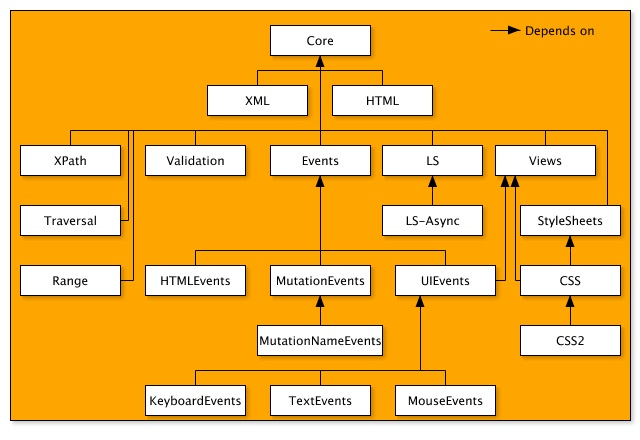
\includegraphics[width=0.65\textwidth]{figures/dom-architecture.jpg}
        \caption{Arquitectura de DOM \cite{w3c}}
        \label{fig:DOM}
    \end{figure}
            
    La interfaz de \textit{DOM} fue definida por el \textbf{OMG IDL} y fue construida para ser usada en una gran variedad de ambientes y aplicaciones. El documento parseado por DOM se transforma en un gran objeto, tal modelo captura la estructura del documento y el comportamiento de éste, además de otros objetos de lo que puede estar compuesto y las relaciones entre ellos. Cada uno de los nodos representa un elemento parseado del documento, el cuál posee una cierta funcionalidad e identidad. La estructura de árbol del DOM construido puede llegar a ser gigantezca, y almacena más de un árbol por cada documento que parsea. 
            
    \subsection{Javascript, VBScript y others}
    \label{chap2:JS}
    Ambos son lenguajes de scripting orientados a objetos. Javascript fue desarrollado por Netscape mientras que VBScript fue desarrollado por Microsft para Internet Explorer, los dos siguen el estandar del lenguage de scripting \textbf{ECMAScript}. Dado que VBScript no era usado por muchos y no tenía soporte para otros navegadores más que Internet Explorer, Microsoft decidió abandonarlo.

    Muchos piensan que JavaScript es un lenguage interpretado, pero es más que eso. Javascript es un lenguage de \textbf{scripting dinámico} (por tanto no tipificado) que soporta la construcción de objetos basados en \textbf{prototipos}. Esto quiere decir que a diferencia de un lenguage de programación orientado a objetos como Java, un lenguage orientado a prototipos no hace la distinción entre clases y objetos (clase instanciada), son simplemente objetos. Y cómo tal al ser construido con sus propidades iniciales, es posible poder agregar o remover propiedades y métodos de forma dinámica (durante el runtime) tanto a un objeto como a la clase.
            
    Javascript puede funcionar tanto como un lenguage de programación procedural o como uno orientado a objetos. Firefox usa una implementación en C de Javascript llamada \textit{Spider Monkey}, Google Chrome/Chromium tiene un motor de JavaScript llamado \textit{V8} e Internet Explore no usa realmente JavaScript si no que \textit{JScript} (hace lo mismo que las otras implementaciones solo que difiere en el sistema operativo que utiliza) que en este caso se llama \textit{Chakra}.
            
    Si bien es posible comprender que JavaScript posee increíbles posibilidades para la creación de \textit{RIA} (Rich Internet Applications), en \cite{barth2009attacks} se muestra que puede llegar a ser un fracaso si es que no se toman en cuenta ciertas vulnerabilidades inherentes al lenguage. Estas vulnerabilidades que pueden llegar a ser criticas, a menudo permiten a un comunicante comprometer completamente a la otra parte. La misma naturaleza de JavaScript que permite la modificación en runtime de los objetos, puede llegar a ser aprovechada de esta situación; en la cita toma por ejemplo la comunicación entre los elementos de un \textit{Mashup}.


    \subsection{Geolocalization}
    Cada Browser posee una API que permite obtener la data de la localización del host donde el browser está alojado. Ésta es obtenida ya sea del GPS, si es un dispositivo móvil, como de la triangulación de la señal del celular, localización de IP del movil o \textit{access point}.


    \subsection{Speedy o SPDY Protocol}
    \label{chap2:spdy}
    Es un protocolo de red abierto desarrollado por Google en el 2009, para el transporte de contenido Web. A modo general utiliza técnicas de \textit{multiplexing}, compresión y prioritización, sin embargo depende bastante de las condiciones del sitio web y su despliegue en la red. SPDY manipula el tráfico en el protocolo HTTP para disminuir el tiempo de carga de las páginas web, al mismo tiempo que cuida la seguridad de los datos. Este protocolo modifica la forma en que las peticiones y respuestas HTTP son enviadas a la internet (por el cable); SPDY es considerado una especie de tunel. Sin embargo, cuando la versión 2 de HTTP esté completa SPDY será deprecada. Implementaciones de este protocolo se dan en: Google Chrome/Chromium, Internet Explorer, Firefox, Safari, Opera y Amazon Silk.

    \subsection{WebWorkers}
    \label{chap2:WWs}
    Ésta tecnología permite la creación de \textit{threads} en el browser para separar las tareas de éste, dejando algunas en el \textit{background} para incrementar el rendimiento total de la carga de las páginas web. Existen 2 tipos: una que es compartida por todo aquello de un mismo \textbf{Origen} y otra que se comunica hacia atrás a la función que la creó. Esta API entrega al desarrollador más flexibilidad, pero que sin duda los atacantes también aprovechan bastante.

    \subsection{CORS: Cross-Origin Resource Sharing}
    \label{chap2:CORS}
    Cómo lo define su nombre es un mecanismo (especificación) que permite al cliente realizar request entre sitios de diverso \textit{Origen}, ignorando el \textbf{SOP}. \textit{CORS} define una forma en que el Browser y el Servidor Web puedan interactuar para determinar si permitir o no el request a otro origen. Un Browser utiliza SOP para restringuir los request de la red y prevenir al cliente de una Aplicación Web ejecutar código que se encuentra en un origen distinto, además de limitar los request HTTP no seguros que podrían tratar de generar un daño. CORS extiende el modelo que el Browser maneja e incluye:
        
        \begin{itemize}
            \item Un header en la respuesta/response del servidor solicitado llamado \textit{Access-Control-Allow-Origin}, donde se debe escribir el origen que tendrá acceso a los recursos solicitados al servidor. Si el valor de la respuesta del servidor coincide con el \textit{origen} de quién lo solicitó, se podrá realizar el uso del recurso en el navegador, de lo contrario se generará un error.

            \item Otro header llamado \textit{Origin} pero esta vez en el request de la solicitud, para permitir al Servidor hacer cumplir las limitaciones en las peticiones de distinto origen.

            \item En algunos casos un browser deberá agregar el header \textit{Access-Control-Allow-Methods}, ya que el servidor no responderá de vuelta si no es así. Esto permite limitar la superficie de ataque en el servidor.

        \end{itemize}
        Existen ciertos métodos en HTTP que necesitan realizar un \textit{pre-vuelo} antes de ser ejecutados, si la response del servidor es afirmativa luego se enviará el request original con el método que se debió confirmar su utilización. Para el caso de los métodos GET y POST, los más usados, este pre-vuelo no es necesario y se puede enviar el request inmediatamente.
        
        La gran diferencia de CORS con cualquier otro método de que permita hacer request hacia un origen distinto, es que el Browser por default no enviará ningún tipo de información que permita identificar al user. De esta manera se puede disminuir considerablemente las amenazas en la confidencialidad, pues el atacante no podrá hacerse pasar por un usuario del que no tiene información. Casi todos los navegadores web, a diferencia de Internet Explore \cite{bookWebAppSec}, realizan sus solicitudes a servidores de diverso origen por medio de la interfaz \textit{XmlHttpRequest}, en el caso de Internet Explorer esta se llama \textit{XDomainRequest}.


    \subsection{Sandboxing}
    \label{chap2:Sandboxing}
    La idea es encapsular el área de mayor probabilidad de ataque en un espacio aislado, minimizando la superficie de ataque de un software. Sandboxing no es una técnica tan nueva, han existido sistemas que ya lo han incorporado. Ésta protección puede ser aplicada dependiendo del diseño del software, algunos ocupan Sandbox a nivel del sistema operativo como otros que ocupan al nivel del \textit{engine} de Javascript. En el caso especial del Browser, esta técnica es construida en el nivel más alto posible para un programa de usuario, lo que permite la separación de privilegios entregados por el sistema operativo al browser y los subprocesos que corren dentro de éste. El atacante que se enfrente a un browser que tenga este mecanismo de defensa, tendrá que realizar primero un \textit{bypass} encontrando una vulnerabilidad en el sandboxing del browser. Existen diferentes técnicas para Sandboxing, todo depende del diseño del Browser.


%%%%%%%%%%%%%%%%%%%%%%%%%%%%%%%%%%%%


\section{Reference Architecture (RA)}
\label{chap2:ArqRef}
%usar \cite{Avgeriou2003}

Una arquitectura de Referencia, de acuerdo a la \textit{Open Security Architecture} o OSA\cite{openSecArch}, es considerado un elemento que describe un \textbf{estado de ser} y debe representar aceptadas buenas practicas. En \cite{Avgeriou2003} se explica que una RA es una arquitectura de software genérica y estandarizada, para un dominio particular e independiente de la plataforma o detalles de implementación. En ésta especifica la decomposición del sistema en subsistemas, las interacciones entre éstas partes y la distribución de funcionalidad entre ellas \cite{Bass2012}. Una RA es una herramienta que permite facilitar el entendimiento de sistemas complejos y su apropiada construcción a sistemas reales. Si bien una RA es usada principalmente para capturar los \textit{concerns} de los \textit{Stakeholders} al comienzo de un Desarrollo de Software, también puede ser usada para educar al realizar la unión de ideas y terminologías usadas por diversos sistemas que se asemejen. Para describir la Arquitectura de Referencia nos hemos basado en los trabajos \cite{Avgeriou2003,Hashizume2014Reference, Submitted2014}, usando patrones para la contrucción de la AR.

Actualmente no hay un consenso de lo que una AR debe contener, \cite{Avgeriou2003} describe un ejemplo e indica como debería de ser ésta con los siguientes elementos:
\begin{itemize}
    \item Describir los Stakeholders que interactuan con el sistema y que poseen \textit{concerns} de éste.
    \item Generar \textit{views} usando UML y teniendo en cuenta un proceso \textit{Rational Unified Process}: crear casos de uso, modelos de análisis y diseño, modelo de despliegue e implementación.
    \item Patrones de Arquitectura.
    \item Atributos de calidad deseables que el sistema debe garantizar. Es importante solo destacar aquellos realmente necesarios, dado que un sistema sobrecargado con ellos tampoco es conveniente.
\end{itemize}

La Arquitectura de Referencia debe ser en lo posible descrita de la forma más abstracta posible, pues su función guiar la construcción de arquitecturas concretas, sin tener en cuenta detalles de las tecnologías usadas.

Las ventajas y usos que se obtienen al construir una RA son:
\begin{itemize}
    \item Comprender la estructura subyacente de un Web Browser y las interacciones que tendrá con otros sistemas.
    \item Proveer una base tecnológica modular y flexible. Al tener los subsistemas compartimentalizados es posible quitar y sacar piezas, que poseen interfaces similares, y de esa manera reusar lo otro sin tener que construir un sistema nuevo.
    \item Entrega una base para el desarrollo de otros Navegadores Web, sin explicar detalles de implementación.
\end{itemize}

En este trabajo el enfoque estará en el primer punto, donde se quiere entender las interacciones entre un desarrollo de Software y la utilización de las funcionalidades del Navegador. Dado que parte de la investigación es obtener Patrones de Mal Uso o Uso Indebido del Navegador Web, es primordial concebir una Arquitectura de Referencia que permita encontrar donde es posible aplicar Patrones de Seguridad para poder mitigar los malos usos del Browser \cite{Submitted2014}. A continuación se presenta la AR obtenida a partir de los Browsers más usados actualmente \cite{statBrow}: Google Chrome/Chromium, Internet Explorer y Firefox.

\section{Secure Software Development and Secure Software Design}
\label{chap2:SSD}

La filosofía detrás de \textit{Secure Software Developmet} es que detrás de cada etapa de desarrollo del software, se tengan en cuenta los prinicipios de Seguridad: Confidencialidad, Integridad, Disponibilidad y Auditoría. Para cumplir este cometido es que se deben llegar a políticas y reglas que aseguren la Seguridad como una propiedad sistémica.

Varias comunidades tienen diferentes enfoques y técnicas de cómo asegurar la Seguridad en los sistemas, muchas pueden incluso tener similitudes y hasta trabajar juntas. En este trabajo, el enfoque tomado es aquél que busca entregar la propiedad de seguridad a través del entendimiento de un sistema a un alto nivel, identificando las amenazas durante la elicitación de requerimientos, de manera que se pueda extraer las posibles amenazas que podrían existir y utilizando elementos de diseño para hacer cumplir los principios de seguridad necesarios por el sistema; este enfoque es el que se dedica la comunidad de \textit{Secure Software Design}. 

Fernandez \cite{fernandez2013security} sostiene que para construir un sistema seguro es necesario realizarlo de manera sistemática de tal manera que la seguridad sea parte del integral de cada una de las etapas del Desarrollo de Software - de inicio a fin. El enfoque que propone es ingenieril y por tanto es aplicable incluso para sistemas \textit{legacy}, donde es posible hacer ingeniería inversa para comprobar si existen o no los requerimiento de seguridad implementados, de manera que permite generar un estudio con la intención de comparar y mejorar nuevos sistemas. En su libro \cite{fernandez2013security} presenta una completa metodología para construir sistemas seguros a partir del Diseño Orientado a Objetos, UML y patrones, a los cuales nombra como \textbf{Security Patterns}.

Como parte de la metodología propuesta, se plantea que para diseñar primero se deben entender las posibles amenazas a las que está expuesto el sistema. La identificación de Amenazas \cite{braz2008eliciting,fernandez2006defining} es la primera tarea que presenta la metodología, que considera las actividades en cada caso de uso del sistema.


\section{Patterns}
\label{chap2:Patt}
Los Patrones encapsulan soluciones recurrentes a problemas y definen una forma de expresar los requerimientos y soluciones de una forma concisa, al mismo tiempo que proveen de un vocabulario común entre los diseñadores \cite{buschman1996system}. Un patrón encarna el conocimiento y experiencia de desarrolladores de software que puede ser reusado posteriormente en nuevas aplicaciones \cite{fernandez2004methodology, fernandez2013security}. Los Patrones expresan las relaciones entre un contexto, un problema y una solución. Para un contexto dado, el patrón puede ser adaptado para encajar en diversas situaciones. La construcción de Patrones de Seguridad parte de la premisa anterior, éste permite construir sistemas seguros a través del uso de Patrones adaptados a las necesidades del sistema y preocupaciones de los \textit{Stakeholders}. Por otra parte, una Arquitectura puede ser descrita a través de Patrones, permitiendo que haya un mejor entendimiento al momento de proveer con guías de diseño y análisis a desarrolladores.

Los patrones describen diseños recurrentes en un mediano nivel de abstraction y es poco probable que existan solos, es decir, existen en conjunto a otros patrones. Un patrón puede proveer una solución usando diagramas en UML, de manera que describen de forma precisa al sistema.

La Arquitectura de Referencia a confeccionar será realizada por medio de patrones y éstos serán descritos con el template creado por \cite{buschman1996system}, llamado POSA, que contiene las siguientes secciones para describir un patrón: \textit{Intent}, Contexto, Problema, Solución, Implementación, Usos comúnes, Consecuencias y Patrones relacionados.




\section{Security Patterns}
\label{chap2:SecPatt}
Los Patrones de Seguridad son aquellos que encarnan buenos principios de diseño que tienen en cuenta ciertos principios de seguridad, y que al ser aplicados en una metodología para el desarrollo de sistemas, es posible asegurar que el sistema aplique esos principios y en consecuencia generar un sistema seguro \cite{fernandez2004methodology, fernandez2013security}. Estos patrones describen las maneras de detener o mitigar una posible amenaza de seguridad, especificando una solución a través de mecanismos de seguridad, para el contexto dado. Las soluciones propuestas deben resolver las fuerzas o \textit{forces} indicadas por el patrón. Un uso importante de estos patrones es la ayuda que aportan a desarrolladores que no son expertos en seguridad; éstos permiten ayudarlos a implementar mecanismos que implementen los principios de seguridad necesarios.

\section{Patrones de Mal Uso}
Para diseñar sistemas seguros, se es necesario identificar las posibles amenazas que un sistema puede sufrir. Papers como \cite{fernandez2006defining, fernandez2007attack, braz2008elicitin, fernandez2013security} describen el desarrollo de una metodología completa para encontrar amenazas, a través del análisis de actividaddes de los casos de uso del sistema buscando como podría un atacante interno o externo socavar las bases de esas actividades. Es importante no confundir \textit{Attack Patterns} con \textit{Misuse Pattern}, pués claramente en \cite{ModMisusePatt, fernandez2013security} dejan explícito que un \textit{Attack Patttern} es una acción que lleva a un mal uso o \textit{misuse}, o acciones \textbf{específicas} que toman ventaja de las vulnerabilidades de un sistema, como por ejemplo un \textit{buffer overflow}. A partir de los trabajos \cite{fernandez2007attack, yoshioka2006development, yoshioka2007integration}  se hace la unión de los conceptos de \textit{Attack Patttern} para dar forma a la definición de \textit{Misuse Pattern} \cite{ModMisusePatt, pelaez2009misuse, fernandez2010worm, hashizume2011misuse, munoz2011misuse, fernandez2012misuse, alkazimi2014, encinamisuse}:
\begin{center}
    Un patrón de mal uso o \textit{Misuse Pattern} describe, desde el punto de vista del atacante, cómo un tipo de ataque es realizado (qué unidades usa y cómo), analiza las maneras de detener el ataque através de la enumeración de posibles Patrones de Seguridad que pueden ser aplicados, y describe cómo rastrear un ataque una vez que ha ocurrido por medio de una recolección y observación apropiada de datos forenses.
\end{center}

Sin embargo, cuando un sistema ya está diseño y construido, como es el caso del Web Browser, lo que va a importar es saber \textbf{cómo} los componentes del sistema, pueden ser usados por el atacante para alcanzar sus objetivos. Un \textit{Misuse Pattern} o \textbf{Patrón de Mal Uso} describe, desde el punto de vista del atacante, cómo un tipo de ataque es realizado, indicando \textbf{qué} componentes usa y \textbf{cómo}. Además analiza las formas de detener el ataque a través de un listado de posibles \textit{Security Patterns} o \textbf{Patrones de Seguridad} que pueden ser aplicados para esa situación, y describe cómo poder seguir el rastro de un ataque una vez que ha sido realizado con éxito en el sistema, a través de data forense. Además describe un contexto en dónde puede ocurrir el ataque.

Un catálogo de \textit{Misuse Patterns} podría ser de gran valor en el Desarrollo de Sistemas que interactúan con el Navegador, pués provee a desarrolladores un medio para evaluar los diseños de sus sistemas, al analizar las posibles amenazas del Browser que pusieran afectar al software que está siendo construído.

\newpage
\chapter{State of Art of Web Browser} %buscar referencia
%LO EXISTENTE EN PAPERS, WEB, ETC. SOBRE EL TEMA DEÑ BROWSER!! MINIS-RESUMENES!!
\label{chap3:EA}
\section{Current Web Browsers}
\label{chap3:BrowExis}

    \subsection{Google Chrome/Google Chromium}
    \label{chap3:GC}
    La misión de Google es organizar la información del mundo y lograr que sea útil y accesible para todo el mundo. Esta gran empresa partió como un búscador y rápidamente llegó a ser dueño de la mayor parte de búsquedas del mercado. Tiene servicios de almacenamiento en la nube, correo electrónico, \textit{e-wallet} y otros más. Google ha sido responsable por la construcción del Navegador Web \textbf{Google Chrome} y \textit{Google Chromium}. En el 2008, Google liberó gran parte del código de Chrome bajo el proyecto de nombre Google Chromium, el cuál es open-source que permitiría a desarrolladores \textit{third-party}, estudiar el código fuente y ayudar en la implementación para las plataformas Linux y OS X. La diferencia entre Chrome y Chromium son: actualizaciones automáticas y Adobe Flash integrado. Así como se puede ver en \cite{EvolutionofWeb} éste Navegador ha sido el último que ha salido y se llevado una gran parte del mercado \cite{statBrow}.

    La arquitectura de Chrome o Chromium se basa principalmente en dos módulos: el Browser Kernel y el Rendering Engine, cómo se puede ver en la Figura \ref{fig:archG}.

    \begin{figure}[h!t]
        \begin{center}
            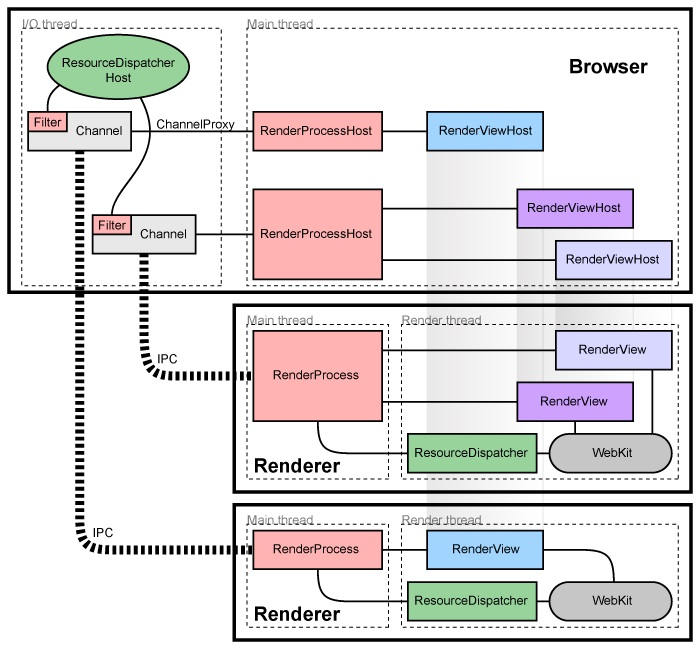
\includegraphics[scale=0.5]{figures/archGC.jpg}
          %\caption{Representación conceptual de una Nube con Eucalyptus. La especificación de las partes y su explicación se ve en \ref{sec:chap2.4.2}. Fuente \cite{EucalyptusOverview}}
          \label{fig:archG}
        \end{center}
    \end{figure}

    Én la documentación de Google Chromium \cite{multiProcArchG}, que es base para Google Chrome, afirma que la arquitectura soporta para cada tab un proceso nuevo, de manera de hacer al Browser más robusto y modularizar el sistema para evitar ciertas amenazas de seguridad. El proceso principal es llamado \textit{Browser Process/Kernel/Engine} y se encarga de la \textit{User Interface}, manejo de las tabs y los procesos de los \textit{plug-in}. Cada tab es asociado a un Rendering Engine, éstos tienen restricciones de acceso (\textit{Sandoboxing}) a los demas y al sistema, lo que permite que exista una protección de la memoria y un control de acceso. En \cite{barth2008security} se explica que el objetivo principal de esta arquitectura es poder mitigar ataques muy severos sin tener que sacrificar la compatibilidad con los sitios web ya existentes. Para lograr el objetivo Google ha ganado muchas lecciones de cómo realizar esto \cite{reis2009browser}, pues explican que un gran desafío en la seguridad es proteger a los usuarios de los atacantes que se aprovechan de las vulnerabilidades y debilidades de los clientes web-browsers. En su arquitectura modular se puede ver que se intenta proveer una seguridad que evita afectar la compatibilidad con otros sitios. La arquitectura comentada se basa en dos decisiones de diseño: La arquitectura depende en el Rendering Engine para aquellos componentes de alto riesgo como JavaScript, el parser de HTML y la creación de DOM para hacer cumplir SOP; al estar rodeados por un Sandboxing hace que el Rendering Engine se comporte como una caja negra. 


    Google Chrome expone en \cite{reis2009browser} que existen ciertas lecciones que han ido utilizando para mejorar la calidad de su browser. Estas son:

    \begin{itemize}
    	\item Reducción de las vulnerabilidades de seguridad, se basa en la aislación de ciertos componentes y la reducción de privilegios de ciertas tareas en el browser. La aislación lo lograron con la creación del Rendering Engine y el Browser Kernel, que tienen como objetivo proteger la data del sistema de archivos. Si bien esto puede no entregar muchos beneficios a una aplicación web, si lo hace en el usuario del browser.
    	\item Reducir la ventana de vulnerabilidades, la actualización del browser se hace cada cierto tiempo de forma automática para así cubrir las vulnerabilidades que van apareciendo.
    	\item Reducción de la frecuencia de exposición, Google trabaja con StopBadware.org para entregar una mayor seguridad al descubrir nuevos tipos de ataques y vulnerabilidades relacionadas con el browser.
    \end{itemize}


    %     \begin{figure}[h!t]
    %     \begin{center}
    %         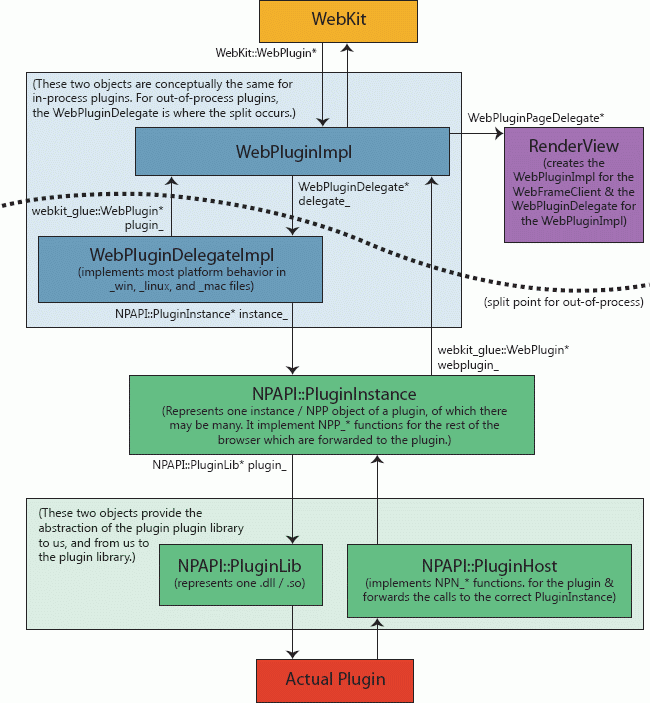
\includegraphics[scale=0.5]{figures/in_process_plugins.png}
    %       %\caption{Representación conceptual de una Nube con Eucalyptus. La especificación de las partes y su explicación se ve en \ref{sec:chap2.4.2}. Fuente \cite{EucalyptusOverview}}
    %       \label{fig:archG}
    %     \end{center}
    % \end{figure}


    % \begin{figure}[h!t]
    %     \begin{center}
    %         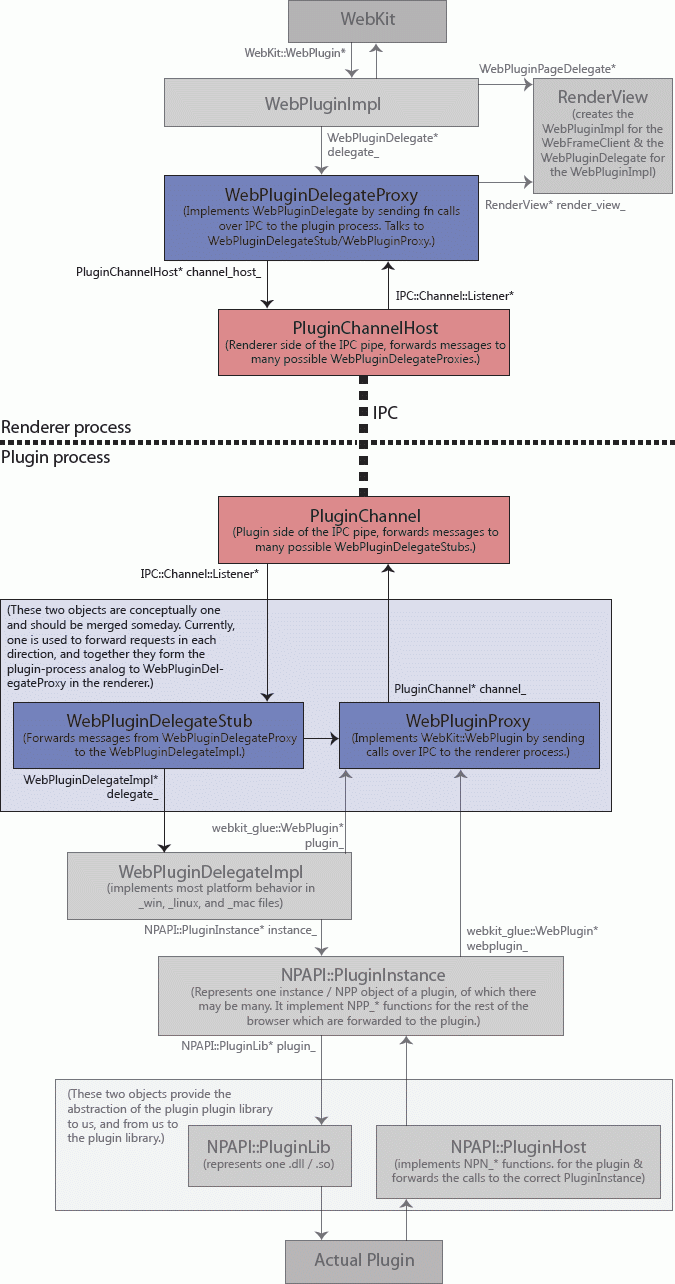
\includegraphics[scale=0.5]{figures/out_of_process_plugins.png}
    %       %\caption{Representación conceptual de una Nube con Eucalyptus. La especificación de las partes y su explicación se ve en \ref{sec:chap2.4.2}. Fuente \cite{EucalyptusOverview}}
    %       \label{fig:archG}
    %     \end{center}
    % \end{figure}

    % \begin{figure}[h!t]
    %     \begin{center}
    %         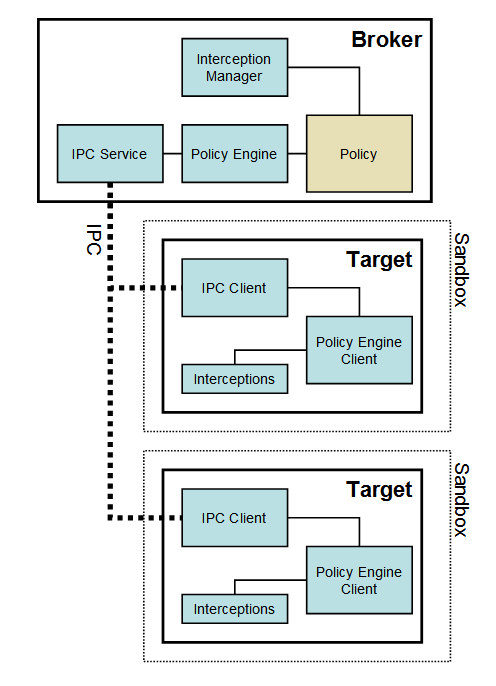
\includegraphics[scale=0.5]{figures/sbox_top_diagram.png}
    %       %\caption{Representación conceptual de una Nube con Eucalyptus. La especificación de las partes y su explicación se ve en \ref{sec:chap2.4.2}. Fuente \cite{EucalyptusOverview}}
    %       \label{fig:archG}
    %     \end{center}
    % \end{figure}




    \subsection{Internet Explorer}
    \label{chap3:IE}
    Internet Explorer es el navegador grafico predeterminado por Microsoft y que su primera versión 1.0 fue realizada en 1995. IE es una derivación de Spyglass Mosaic desarrolado por la NCSA (National Center for Supercomputing Applications). En primera instancia fue un navegador que podría ser obtebido si era comprado como complemento de \textit{Microsoft Plus!} o mediante la versión \textit{OEM} de Windows 95. Desde la tercera versión de IE, en 1996, que esta se lanzó de forma gratuita.
            
    La arquitectura de este navegador es modular y permite al desarrollador por utilizar los recursos para crear diferentes funcionalidades, ejemplo de esto son: toolbars, Microsoft Active X controls, etc. En la Figura \ref{fig:archIE} \cite{IEArch} se puede ver los principales componentes de la architectura del browser mencionado. IE utiliza \textit{COM} o \textit{Component Object Model} una interfaz binaria standard para componentes de software introducida por Microsoft en 1993 y que permite una comunicación entre procesos/componentes de software provenientes de la familia de software de Microsoft. \textit{COM} es similar a otras tecnologías de interfaz de componentes de software ( Component Software Interface Technologies) cómo CORBA y Java Beans. El uso de \textit{COM} gobierna la forma la interacción de los componentes que se comunicann y permite que haya un reuso y extensibilidad de estos.
            
    \begin{figure}[h!t]
        \begin{center}
    		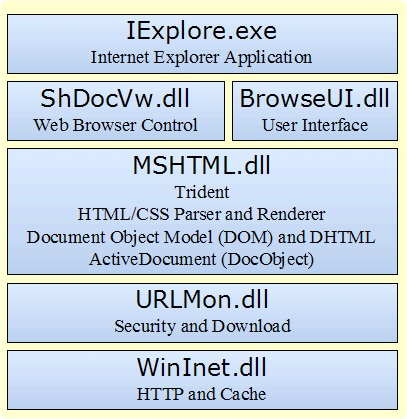
\includegraphics[scale=0.65]{figures/IEArch.jpg}
          %\caption{Representación conceptual de una Nube con Eucalyptus. La especificación de las partes y su explicación se ve en \ref{sec:chap2.4.2}. Fuente \cite{EucalyptusOverview}}
          \label{fig:archIE}
        \end{center}
    \end{figure}
   
   \subsubsection*{Rendering Engine}   
   \label{chap2:Trident}
   O también llamado MSHTML, es un rendering engine privativo, sin embargo es posible usarlo al usar librería de Windows \textbf{mshtml.dll}. Según \cite{Crowley2010} es un objeto OLE (Object Linking and Embedding) Active Document que representa el \textit{layout} de Internet Explorer y permite mostrar graficamente las páginas por medio del \textit{display} del host. Dentro de éste se manejan las Extenciones, el \textit{engine} de Javascript y la librería que contiene la API para tareas de \textit{networking}, además de proveer una capa de seguridad y manejar las descargas de archivos.



    % \begin{figure}[h!t]
    %     \begin{center}
    %         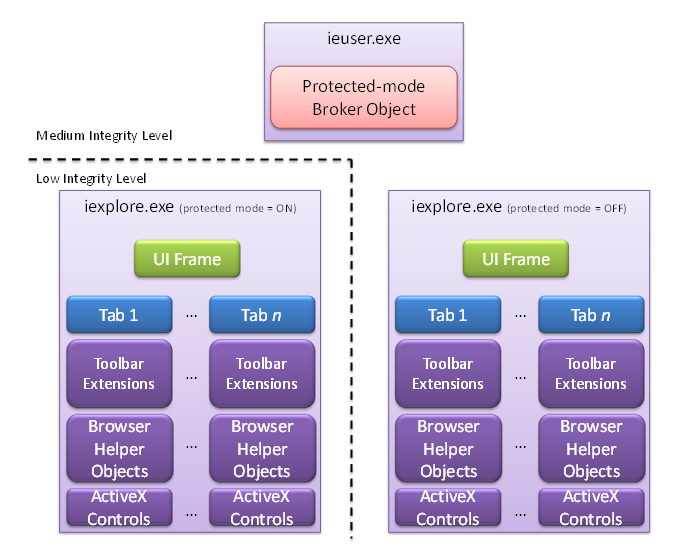
\includegraphics[scale=0.5]{figures/11_IE8andLooselyCoupledIELCIE_1.png}
    %       %\caption{Representación conceptual de una Nube con Eucalyptus. La especificación de las partes y su explicación se ve en \ref{sec:chap2.4.2}. Fuente \cite{EucalyptusOverview}}
    %       \label{fig:archG}
    %     \end{center}
    % \end{figure}


    % \begin{figure}[h!t]
    %     \begin{center}
    %         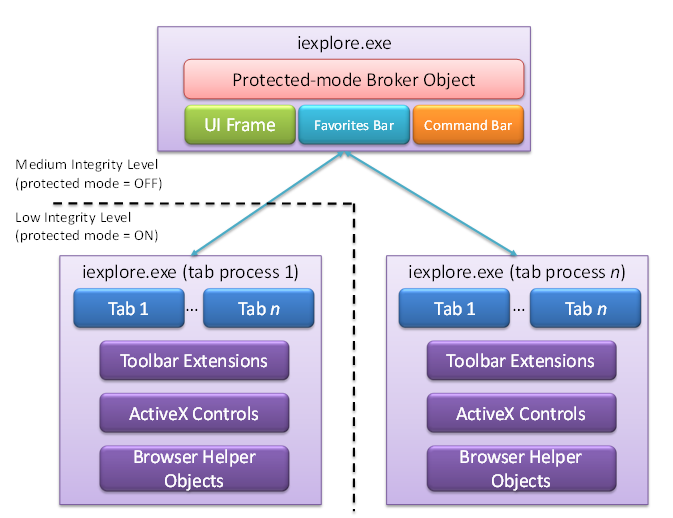
\includegraphics[scale=0.5]{figures/11_IE8andLooselyCoupledIELCIE_2.png}
    %       %\caption{Representación conceptual de una Nube con Eucalyptus. La especificación de las partes y su explicación se ve en \ref{sec:chap2.4.2}. Fuente \cite{EucalyptusOverview}}
    %       \label{fig:archG}
    %     \end{center}
    % \end{figure}


    \subsection{Firefox}
    \label{chap3:Firefox}

    Firefox fue creado a partir del navegador \textit{Netscape} en 1998, actualmente la fundación Mozilla ha sido la que la ha mantenido, generando varias modificaciones desde su nacimiento. Las metas de diseño que Mozilla desee en el navegador son:
    \begin{itemize}
        \item Renderizado rápido de las páginas web.
        \item Fuerte apoyo a los estandares web como la W3C.
        \item Interoperabilidad en las diversas plataformas.
    \end{itemize}

    \begin{figure}[h!t]
        \begin{center}
    		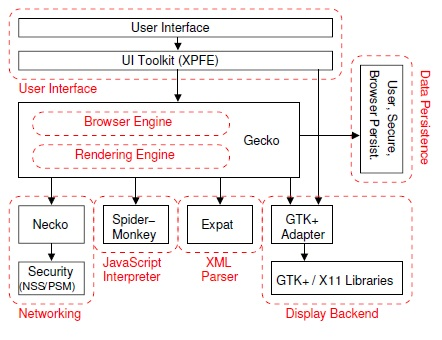
\includegraphics[scale=0.8]{figures/archMoz.jpg}
          %\caption{Representación conceptual de una Nube con Eucalyptus. La especificación de las partes y su explicación se ve en \ref{sec:chap2.4.2}. Fuente \cite{EucalyptusOverview}}
          \label{fig:archM}
        \end{center}
    \end{figure}
            
    La arquitectura de este browser puede ser vista en la Figura \ref{fig:archM} donde se pueden observar los siguientes componentes:
            \begin{itemize}
                \item La interfaz de usuario, puede ser reutilizada para otras aplicaciones.
                \item La persistencia de los datos, tanto de bookmarks como de data de bajo nivel como el \textit{cache}.
                \item EL \textit{Rendering Engine}, permite el renderizado de documentos HTML/XML aún cuando estos estén mal formados. Este Engine es capaz de renderizar la interfaz de la aplicación multi-plataforma.
            \end{itemize}
    La arquitectura de Mozilla se distingue de las demás en que la visualización especificada por la plataforma y la librería de \textit{widgets} son usados directamente en el navegador, lo que minimiza el costo necesario para soportar diferentes plataformas.
            



\section{Reference Architecture and Patterns}
\label{chap3:ArqRefBrowandPatt}
%Referirme a los artículos que hayan realizado antes el trabajo
%usar: 2005-grosskurth-browser-refarch, preprint-grosskurth-browser-archevol, webpag3 (IE), reis2009isolating
%usar Larrondo 535061 (análisis de dominio del web browser)
% Godfrey2000 extrae architectura de software de Firefox

%Decir: "este trabajo es basado en la metodología de Fernandez \cite{Hashizume2014Reference} usando patrones en la construcción de la arquitectura de referencia"


%larrondo
En Larrondo-Petrie et. al \cite{535061} se realiza un análisis orientado a objetos del dominio del web browser, con el fin de obtener un modelo de dominio, un modelo de objetos y un \textit{feature tree} que describiera la estructura y funcionalidad entregada comúnmente por los Web Browser. Sin embargo éste estudio está bastante lejos de lo que se quiere hacer en este trabajo, sin embargo sirve para obtener un transfondo de lo que sucede en el Web Browser, aún cuando la información esté muy desactualizada.

% preprint-grosskurth-browser-archevol y 2005-grosskurth-browser-refarch

En el trabajo de Grosskurth et al. \cite{2005-grosskurth-browser-refarch, preprint-grosskurth-browser-archevol} se llega a una arquitectura de referencia de muy alto nivel en base a dos navegadores open-source: Mozilla y Konqueror. En esta arquitectura se identifican los siguientes subcomponentes: Interfaz Usuaria, Persistencia de Datos, Browser Engine, Rendering Engine, Networking, Interprete de Javascript, XML Parser y Display Backend. Una vez obtenida la parte conceptual, se inició una evaluación de ésta al comparar las arquitecturas concretas de cada browser open-source, obtenidas por una herramientas de ingeniería inversa, para ver que tanto el modelo conceptual era cercano a la realidad; los browsers usados para validar fueron: Epiphany, Safari, Lynx, Mosaic y Firefox. Si bien la arquitectura entregada entrega bastante información a alto nivel, no desarrolla más que esa capa de abstracción. Además explica cada subsistema con los elementos que se deberían encontrar y para que son usados, por ejemplo explica que en el Rendering Engine es el encargado de mostrar lo parseado del HTML o XML de la página web e indica la relación de éste con el Browser Engine. 


%Godfrey2000
En el documento \cite{Godfrey2000} realizado en el año 2000, se describe la experiencia realizada al extender el rabajo del proyecto TAXFORM. Usando PBS, una herramienta de Ingeniería Inversa, se extrajo la arquitectura de software del Navegador Mozilla, con el objetivo de entender la estructuración de sus componentes. Si bien el trabajo ayuda a entender un poco la estructura detrás del navegador, este trabajo es muy antiguo y la versión más actual del navegador ha cambiado bastante. Además lamentablemente, el enfoque de este estudio no es intentar entender lo que hace cada subsistema, si no que es la implementación de la herramienta misma para obtener la arquitectura de software del browser seleccionado.

%Lwin2009 - Agent Based Web Browser
En \cite{Lwin2009} se propone un Browser llamado Anfel SOFT, donde gracias al uso de Inteligencia Artificial, crea agentes que permiten mejorar la experiencia del usuario. El trabajo asegura que el browser será capaz de aprender el comportamiento de navegación del usuario, y guiará al usuario en su navegación para que esta sea lo más efectiva posible. El paper obtiene los subsistemas que se pueden encontrar en un browser de la misma manera que lo realiza \cite{2005-grosskurth-browser-refarch}. Si bien la arquitectura que muestra refleja parte de lo visto en los 3 browsers escogidos en este estudio, no da detalles acerca de cada subsistema identificado. Además la arquitectura de Referencia que entrega es la misma vista en \cite{2005-grosskurth-browser-refarch, preprint-grosskurth-browser-archevol} y a pesar que identifica otros posibles componentes, no agrega nada nuevo.

Podemos ver en los trabajos ya mencionados, que la definición de Arquitectura de Referencia dista bastante de la definición dada por nosotros en el capítulo 2. En cada uno de ellos el trabajo ha sido a muy alto nivel y la descripción de los subcomponetes del sistema es mínima. Si bien explican las relaciones entre éstos, no dan un mayor entendimiento en como se comportan en ciertas situaciones. Desafortunadamente para esta memoria no existe mucha literatura sobre el desarrollo de una Arquitectura de Referencia del Browser, y de lo que hay el trabajo más actual es el realizado por \cite{Lwin2009} en el año 2009.




\section{Evolutions and Security of the Web Browser}
\label{chap3:EvoandSec}
%Usar referencias varga2013evolution, EvoBrowSecNSS, browSecPhish, browSecPrivSett, rowSecSEMBlock, silic2010security, barth2008security, reis2009browser, reis2009isolating, barth2009securing, barth2010protecting, Carlini12, liu2012chrome, utakrit2009review, barth2009secure, Accuvant11, Li12, Yu07, Zalewsk08, alcorn2014browser, sansInstInfoSec, 
% evolucion de la web: http://www.evolutionoftheweb.com/ (infografía)

En \cite{2005-grosskurth-browser-refarch} y \cite{preprint-grosskurth-browser-archevol} podemos notar que existe una mayor importancia en llegar a los componentes y las relaciones detrás del browser, y casi una nula mención de elementos de seguridad que permiten salvaguardar datos críticos o cómo protege al host de las amenazas. Podemos dar esta falta de conocimiento dado que en tales fehcas la cantidad de ataques de seguridad al Browser es mucho menos que en la actualidad %poner referencia.


\subsection{Estandarizaciones}
\label{chap3:Standars}

\subsection{Vulnerabilidades}
\label{chap3:vuln}

\subsection{Amenazas}
\label{chap3:threats}

\subsection{Medidas de Mitigación o Mecanismos de Defensa}
\label{chap3:mitig}

    \begin{enumerate}
        %CHROME/CHROMIUM
        \item Safe Browsing API and Content-Agnostic Malware Prevention
        \\XXX 
        %Lo usa chrome/chromium y FIREFOX!!!
        %Safe Browsing API es inefectiva contra ataques de Social Eng Malware, citas: rowSecSEMBlock
        %Abrams2013:    The NSS analyst brief, “Cybercrime  Kill    Chain   vs. Defense Effectiveness,” demonstrates    that    holes   in  one layer   of  defense are often   not  closed by  secondary   and tertiary technologies. Google   augments    its Safe    Browsing    API with    additional  download    protection  that    is  seven   times   more    effective   than    the Safe    Browsing    API.

        \item Sandoxing
        \\En el desarrollo de \cite{barth2008security} se define un modelo de amenazas donde se enumeran las habilidades que debería de tener un atacante y los objetivos de estos, para así caracterizar y evaluar las propiedades de seguridad necesarias para evitar que los atacantes cumplan su objetivo. Una propiedad importante que hacen destacar en el estudio es cómo aislar ciertos procesos que pueden ser aprovechados por los atacantes y ofrece una forma para poder mitigar esto: Sandboxing. El Sandboxing de Google Chrome previene al atacante de leer o escribir en el sistema de archivos del usuario, dejando al Principal Web con los privilegios necesarios para parsear un HTML/XML y ejecutar código JavaScript. Sin embargo esta arquitectura no imposibilita al atacante a atacar otros sitios web si es que el Rendering Engine fue comprometido, lo que puede convertirse en una amenaza muy grande para otros sitios web.

        \item Actualizaciones Periódicas en Background
        \\XXX

        \item Privacy Settings: Do Not Track and Third-Party Cookies
        \\XXX
        %En los 3 browsers


        %IE
        \item SmartScreen
        \\XXX
        
        \item Application Reputation / App Rep
        \\XXX


        %FIREFOX
        \item Content Security Policy
        \\XXX


        \item HTTP Headers
        \\XXX

    \end{enumerate}



%\section{Diagrama de Clases del Browser}
%Creemos que parte del trabajo que existe en realizar la Arquitectura de Referencia y los Patrones de Mal Uso, es entender la estructura estática del Browser. En la siguiente figura exponemos un diagrama en UML extraído a partir de lo visto en los 3 Navegadores Web que se han investigado: Google Chrome/Chromium, Internet Explorer y Firefox.

    % \begin{figure}[h!t]
    %     \begin{center}
    %         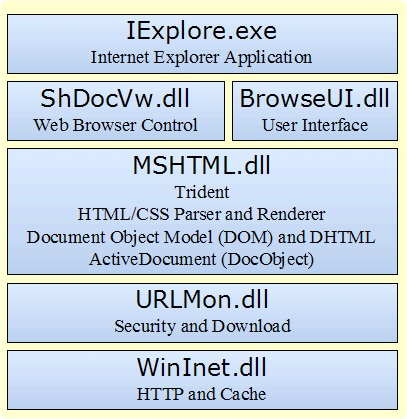
\includegraphics[scale=0.65]{figures/IEArch.jpg}
    %       %\caption{Representación conceptual de una Nube con Eucalyptus. La especificación de las partes y su explicación se ve en \ref{sec:chap2.4.2}. Fuente \cite{EucalyptusOverview}}
    %       \label{fig:archIE}
    %     \end{center}
    % \end{figure}


\section{Sumario}
\label{chap3:Summ}



% \subsection{Rendering Engines}
% \label{chap2:RenderingE}
% Responsable de converitir la página web, en HTML o XML, a un formato visible cómodo para el usuario en la pantalla del host. La combinación de HTML, CSS y media (imagenes, videos, etc.) permiten entregar una experiencia gráfica al usuario con la que interactuará. Existen browser que no usan gráficos y solo se basan en mostrar texto, ejemplos de estos navegadores son: W3M y Lynx. Los \textit{Rendering Engines} más usados son: Webkit (Safari), Blink (Google Chrome/Chromium), Trident (Internet Explorer) y Gecko (Firefox).

%     \subsubsection{Trident}
%     
%     \subsubsection{Gecko}
%     \label{chap2:Gecko}
%     Es un motor de renderizado \textit{Open Source}, escrito en C++, creado en un comienzo por Netscape, predecesor de Mozilla Foundation/Corporation. La función de este componente en Firefox (y otros browsers que lo integran) es leer el \textit{web content} de tipo HTML, CSS, XUL (para renderizar \textit{User Interface}) y Javascript, y mostrarlo al usuario en un formato gráfico. Tiene un gran rendiemiento al transformar a formato gráfico una página con lenguaje de marcado ya que soporta multithreading en el parser de HTML. Gecko fue diseñado para soportar \textit{Open Internet Standards} y por ende sigue al pie de la letra todas las especificaciones de HTML 4, CCS 1 y 2, DOM, XML y Javascript. Los componentes de Gecko incluyen:
%         \begin{itemize}
%             \item Parser de Documentos (HTML y XML).
%             \item \textit{Layout Engine} con un modelo de contenido; ésta es la información que el display del host mostrará al usuario.
%             \item Sistema de estilos.
%             \item Motor de Javascript. En el caso de Gecko éste se llama \textbf{SpiderMonkey} que está escrito en C/C++.
%             \item Librería de imágenes.
%             \item Librería de \textit{Networking}.
%             \item Renderizado gráfico específico a la plataforma y widget de acuerdo al sistema operativo.
%             \item Librerías de Seguridad.
%             \item librería de preferencias de usuario, entre otros más.
%         \end{itemize}

%     \begin{figure}[h]
%         \centering
%         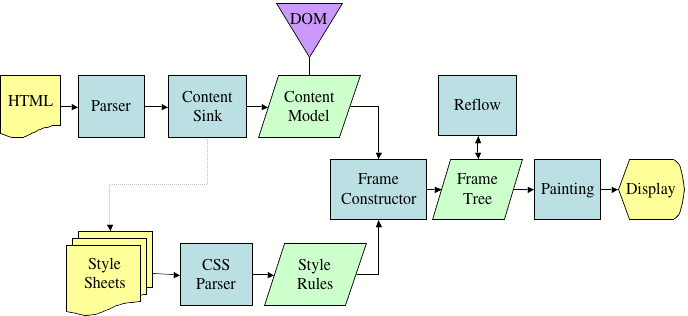
\includegraphics[width=0.8\textwidth]{figures/Gecko_Overview_9.png}
%         \caption{Diagrama de la ejecución de un Rendering Engine \cite{gecko}}
%         \label{fig:DOM}
%     \end{figure}       


%     \subsubsection{Blink}
%     \label{chap2:Blink}
%     Es el \textit{Rendering Engine} usado por Google Chrome/Chromium y es el \textit{forking} del trabajo original llamado Webkit. Su objetivo principal es soportar la architectura de multi-procesos que posee el navegador y al mismo tiempo poder reducir el nivel de complejidad.






\newpage
\chapter{Arquitectura de Referencia del Browser}
\label{chap4:ArqRefBrowser}

La arquitectura de referencia a construir en este trabajo tiene como objetivo catalizar el entendimiento de la estrecha relación que existe entre el \cite{Web Browser} y los sistemas que serían construídos sobre la Internet. En vista a la poca, casi nula, documentación de la creación de Arquitecturas de Referencias del Navegador Web, la necesidad de hacer una AR para entender cómo la arquitectura de este sistema puede relacionarse con el futuro desarrollo de otros sistemas, llega a ser imperante. Al considerar al Web browser como un \textit{concern} en el desarrollo de SoftWare puede ser una buena estrategia para evitar una gran perdida monetaria u organizacional. Se sabe que el Browser es un pieza de Software que ha sufrido varios cambios desde la década de los 90, por lo tanto entre los desarrolladores de ésta herramienta ya existen conveniones de qué elementos funcionan mejor. Por consiguiente, no es de extrañar que diferentes browsers estén construidos de formas muy similares, y en consecuencia puedan ser conceptualizados en una Arquitectura de Referencia que manifeste los componentes, mecanismos de comunicación y funciones de esta pieza de Software.

En este capítulo se presenta una Arquitectura de Referencia (AR) desarrollada principalmente a partir de la abstracción de las propuestas existentes hoy em día como: Google Chrome/Chromium, Internet Explorer y Firefox; nos basaremos en información del año 2014 hacia atrás. Primero se identificarán y analizarán los stakeholders, se identificarán los casos de uso relacionados a uno de estos stakeholders y se dará una descripción breve. Luego se presentarán patrones que formarán parte de nuestra AR. Éstos patrones serán descritos utilizando un template POSA \cite{buschman1996system} y notación UML para precisar cómo los componentes de la AR se relacionan.


\section{Casos de Uso del Browser}
	\subsection{Stakeholders (actores) y Concerns de estos}
	Se es necesario encontrar los actores (definido por sus roles) que participan en el uso y operación del Navegador, estos son:
		\subsubsection{Usuario Consumidor (UC)}
		Este es el principal stakeholder, pues de él depende que se realice el inicio de una petición para buscar una página web, recurso o servicio. Sin éste la utilidad del Web Browser es nula. El stakeholder al mismo tiempo podría ser una entidad no humana, como un plugin, extensión o instancia de una página web, que requiere hacer peticiones por medio de las interfaces del navegador, pero que al fin y al cabo cumplen con los deseo del usuario del host de mostrar el contenido.

		\subsubsection{Sistema Operativo (SO)}
		Crea el o los procesos necesarios para iniciar el Navegador, además de entregar un ambiente al Browser para que éste pueda funcionar adecuadamente. En base al enfoque de este estudio, ésta identidad se encarga de aplicar políticas de seguridad sobre el Browser cuando se necesiten realizar operaciones o el navegador desee crear nuevos procesos.

		\subsubsection{Proveedor de Servicios (PS)}
		Este puede ser un: Web Server, Web Aplicación, Servicio de actualización del Browser, etc. Su interacción con el Browser se limita a entregar contenido a éste, no a usarlo.

	\subsection{Casos de Uso}
	\subsubsection{Casos de Uso para Usuario Consumidor}
		El usuario consumidor es el más importante stakeholder del web browser, pues sin él no habría razón para la existencia del browser; un servidor tampoco existiría dado el mismo principio. Bajo ésta entidad es que suceden la mayoría de los casos de uso del sistema al que realizaremos su AR. Al encontrar los casos de uso de éste stakeholder veremos los concerns de éste, lo que nos permitirá entender las necesidades de seguridad para proteger al navegador.
			\begin{enumerate}
				\item Usar datos privados de usuario (opcional): dependiendo del navegador, se podría indicar al usuario si quiere usar una cuenta externa o interna para acceder a información propia de usuario consumidor y mejor así la experiencia de usuario.

				\item Realizar Petición/Request: El caso de uso más importante de éste sistema y en la que se basa la arquitectura cliente/servidor. Esta acción considera encontrar el recurso bajo la URI dada y la consecuente descarga del recurso. La descarga no es siempre necesaria, pues existe lo que se conoce como una peticiíon \textit{preflight} donde solo se envía una petición para saber si es seguro realizar una petición/request. Entonces como una consideración a este caso de uso es que una petición/request no siempre conlleva una respuesta/response, por lo que hemos condensado estas dos (request/response) en un solo caso de uso. 

				\item Descargar recurso: Este caso de uso está incluído dentro de Petición/Request, pues para conseguir una página web es necesario la descarga del recurso.

				\item Solicitar intervención: exiten oportunidades en que la realización de una petición/request conllevará a que el Browser pida permiso al UC para realizar otras acciones, ejemplo: instalar un plug-in, extensión, descargar un contenido que no se puede evaluar su seguridad. En los casos anteriores, una ventana de la interfaz gráfica pedira explícitamente la intervención del usuario para tomar una decisión.

			\end{enumerate}

		Existen muchos más casos de uso relativos al stakeholder tomado, pero para este trabajo bastarán con los propuestos. Una vez que sabemos los roles involucrados y la forma en que interactuan con el sistema, será posible encontrar las amenazas contra el browser.

		\subsubsection{Casos de Uso para el Sistema Operativo}
			\begin{enumerate}
				\item Operación CRUD en host: Acción realizada cuando el Browser obtiene una solicitud explícita o no (automática), del usuario para realizar acciones que involucren permitir un acceso desde el sistema operativo como: leer, escribir o modificar/eliminar algún recurso del host.

				\item Recibir solicitud: En un browser es normal la comunicación entre los procesos que lo componen y el Sistema operativo por medio de un canal de comunicación, ejemplo de esto es cuando un plug-in se comunica con el proceso encargado de mostrar por pantalla lo que se hace en él.
			\end{enumerate}

		\subsubsection{Casos de Uso para el Proveedor de Servicios}

			\begin{enumerate}
				\item Recibir Petición/Request: El PS siempre está escuchando en sus puertos habilitados a posibles peticiones de sus clientes. Una petición es recibida en un formato que el PS debe saber interpretar y en consecuencia realizar las acciones correspondientes que el cliente le pide. Por cada solicitud del cliente, en este caso el Web Browser, habrá una respuesta/response por parte del PS. Este caso de uso no se ejecuta, si dentro del header de uno de los paquetes está indicado que la petición fue hecha en modo \textit{preflight}.

				\item Operación CRUD: alguna petición podría terminar por realizar un cambio en el PS dado por alguna operación CRUD. Éstas opciones son la voluntad del usuario en el host, y que son transmitidas y realizadas indirectamente por el Web Browser.
			\end{enumerate}

		Los casos de Uso descritos anteriormente se pueden divisar en la Figura \ref{fig:CUBrowser}

	    \begin{figure}[h]
	        \centering
	        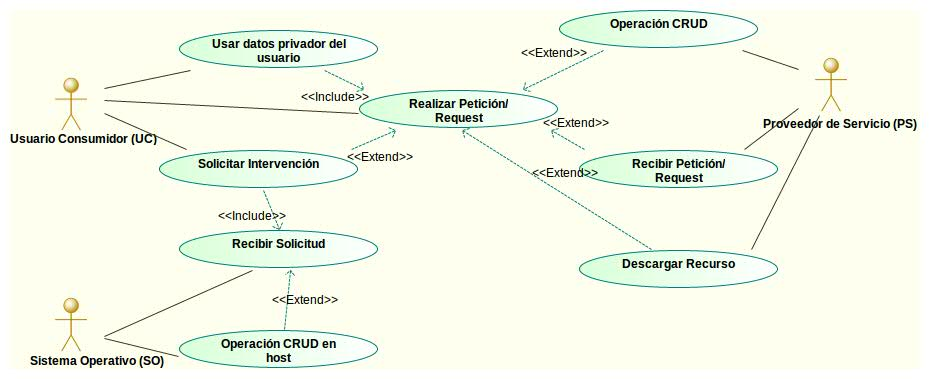
\includegraphics[scale=0.45]{figures/CUBrowser.jpg}
	        \caption{Diagrama de Caso de Uso del Web Browser}
	        \label{fig:CUBrowser}
	    \end{figure}



\section{Patrón Broker/Frame/Browser Engine/Process (BP)}
\label{chap4:BrokerPatt}
\subsection*{Intent}
El patrón Broker/Frame/Browser Engine/Process o BP 


\subsection*{Ejemplo}

\subsection*{Contexto}

\subsection*{Solución}

\subsection*{Estructura}

\subsection*{Dinámica}

\subsection*{Consecuencias}

\subsection*{Ejemplo Resuelto}

\subsection*{Usos Comúnes}

\subsection*{Patrones Asociados}

\newpage

\section{Patrón Rendering Engine (RE)}
\label{chap4:REPatt}
\subsection*{Intent}
El patrón Rendering Engine o RE representa a todos los componentes necesarios para realizar el parsing y layout de HTML y XML, interpretación de javascript, construcción del DOM y las interfaces limitadas para la comunicación entre procesos con el BP, para el posterior display de la información por pantalla usando Sistema Operativo (SO).


\subsection*{Ejemplo}

\subsection*{Contexto}

\subsection*{Solución}

\subsection*{Estructura}

\subsection*{Dinámica}

\subsection*{Consecuencias}

\subsection*{Ejemplo Resuelto}

\subsection*{Usos Comúnes}

\subsection*{Patrones Asociados}

\newpage

\section{Patrón User Interface}
\label{chap4:UIPatt}
\subsection*{Intent}

\subsection*{Ejemplo}

\subsection*{Contexto}

\subsection*{Solución}

\subsection*{Estructura}

\subsection*{Dinámica}

\subsection*{Consecuencias}

\subsection*{Ejemplo Resuelto}

\subsection*{Usos Comúnes}

\subsection*{Patrones Asociados}

\newpage

\section{Patrón Plugin}
\label{chap4:PluginPatt}
\subsection*{Intent}

\subsection*{Ejemplo}

\subsection*{Contexto}

\subsection*{Solución}

\subsection*{Estructura}

\subsection*{Dinámica}

\subsection*{Consecuencias}

\subsection*{Ejemplo Resuelto}

\subsection*{Usos Comúnes}

\subsection*{Patrones Asociados}


\newpage
\chapter{Patrones de Mal Uso}
\label{chap5:MisusePatt}
En este capítulo se tiene como objetivos: obtener las amenazas que afectan al Web Browser y obtener Patrones de Mal Uso o Uso Indebido que las reflejen. Se realizará un análisis de amenazas basada en la metodología \cite{braz2008eliciting}, que busca en base a las actividades de los casos de uso los posibles males usos que podrían realizar los atancates.


\section{Identificando Amenazas}
\label{chap5:IdenThreat}


\section{Template de Patrones de Mal Uso}
\label{chap5:TemplateMP}
Esta sección describe cada parte del template a usar para un Patron de Mal uso o Uso Indebido.

\subsection*{Nombre}
El nombre del patrón debe corresponder al nombre genérico dado al tipo específico de ataque en los repositorios estandares de ataques, como por el usado por el CERT \cite{cve}.

\subsection*{Intent o descripción básica}
Una descripción corta del propósito del patrón (qué problema resuelve para el atacante).

\subsection*{Contexto}
Describe el entorno genérico incluyendo las condiciones bajo a las cuales el ataque puede ocurrir. Esto puede incluir defensas mínimas presentes en el sistema, así como también vulnerabilidades típicas del sistema. El contexto puede ser especificado usando Diagramas de \textit{Deployment} de las partes relevantes del sistema así como también Diagaramas de Secuencia o de Colaboración que explayen el uso normal del sistema. Un diagrama de clases podría mostrar la estructura relevante del sistema. Se especifican además precondiciones para que el ataque ocurra.

\subsection*{Problema}
Desde la mirada del atacante, el problema es encontrar \textbf{cómo} atacar el sistema. Un problema adicional es cuando el sistema está protegido por mecanismos de defensa. Las \textbf{fuerzas o forces} indican qué factores pueden ser requeridos en orden de ejecutar el ataque y en cómo realizarlo; por ejemplo, qué vulnerabilidades pueden ser explotadas. Además, qué factores podrían evitar que el ataque se pueda llevar acabo o lo retrasen.

\subsection*{Solución}
Esta sección describe la solución que resuelve el problema del atacante, ej: cómo el ataque puede alcanzar sus objetivos y los resultados esperados de éste. Diagramas en UML muestran los componentes del sistema involucrados. Diagramas de Secuencia o Colaboración muestran el intercambio de mensajes necesarios para cumplir con el ataque. Diagramas de actividad pueden añadir más detalle.

\subsection*{Componentes del sistema afectados (Dónde buscar evidencia)}
Esta sección adicional al \textit{template} original de un Patrón de Seguridad \cite{fernandez2013security} es nueva, dado que tiene relación con el mal uso realizado. La solución debe representar todos los componentes que están involucrados en el ataque, pero no debe ser una extensa lista, solo los más importantes para prevenirlo o lo escencial para una examinación forense. Esto puede ser representado por un diagrama de clases, que puede ser un subset o un superset del diagrama del contexto.

\subsection*{Usos comúnes}
Incidentes específicos en donde el ataque ha ocurrido son preferidos, pero para vulnerabilidades nuevas, donde el ataque aún puede que aún no se haya realizado, un contexto específico dónde el ataque pueda llevarse acabo es suficiente.

\subsection*{Consecuencias}
Discute los beneficios y desventajas del patrón de mal uso o uso indebido desde el punto de vista del atacante. ¿Es acaso el esfuerzo y costo gastado comparable a los resultados obtenidos? Esta es una evaluación que debe ser realizada por el atacante al decidir realizar el ataque; Diseñadores deben evaluar el riesgo de sus activos usando algpún enfoque de análisis de riesgos. La enumeración incluye buenos y malos aspectos, que deben ser emparejados a las fuerzas o \textit{forces}


\subsection*{Contramedidas y datos Forenses}
Esta sección describe las medidas de seguridad necesarias para detener, mitigar, o rastrear este tipo de ataque. Esto implica la enumeración de los Patrones de Seguridad o \textit{Security Patterns} que son efectivos contra este ataque. Desde un punto de vista Forense, se describe qué información puede ser obtenida en cada etapa rastreando el ataque y lo que puede ser deducido de los datos con el fin de identificar el ataque en específico. Finalmente, podría indicar qué información adicional debe ser recolectada en los componentes o unidades incolucrados para poder mejorar el análisis forense.


\subsection*{Patrones Similares}
Discute otros patrones de mal uso o uso indebido con diferentes objetivos pero realizados de manera similar, o con objetivos similares pero realizados de otra manera.

%\section{Escuchar Tráfico}


%\section{Robo de Datos privados por medio de extensión mal configurada}
\newpage
\chapter{Discusión}
\label{chap6:Disc}
\newpage
\chapter{Conclusiones}
\label{chap7:conclusion}


\section{Contribuciones}
\label{chap7:contrib}

\section{Trabajo Futuro}
\label{chap7:Futuro}

%\backmatter
%\addcontentsline{toc}{chapter}{References}
\bibliography{ref}
\bibliographystyle{unsrt}

\appendix
\chapter{Anexos}
\label{Anexos}

%\label{Anexo2}

\section{asdf}


\end{document}